\documentclass[orivec]{llncs}
\usepackage{graphicx}
\usepackage{amsmath}			% for "cases"
\usepackage{amsfonts}		% for frakur fonts
\usepackage{mathrsfs}		% for curly "E" error symbol
\usepackage{float}
\usepackage{tcolorbox}		% for wrapping example in color box
%\usepackage{wrapfig}			% wrap figure beside text, used in example
\usepackage{tikz-cd}			% commutative diagrams
\usepackage{amssymb}			% for \multimap, \updownarrow, \bigstar
\usepackage{sectsty}			% change section color
%\usepackage{turnstile}		% longer turnstiles
\usepackage{wasysym}			% smileys
%\usepackage{cancel}			% center "not" line for "broken heart"
\usepackage{soul}			% allow line breaking in \underline

% *************** Delete when not using Chinese or colors **********************
\usepackage{xeCJK}
\setCJKmainfont[BoldFont=SimHei,ItalicFont=KaiTi]{SimSun}
\usepackage{color}
\definecolor{Cerulean}{RGB}{100,100,200}
\newcommand{\emp}[1]{\textbf{\textcolor{Cerulean}{#1}}}
\definecolor{grey}{rgb}{0.9,0.9,0.9}  % grey

% \chapterfont{\color{blue}}  % sets colour of chapters
\sectionfont{\color{blue}} 
\subsectionfont{\color{blue}} 
\subsubsectionfont{\color{blue}} 

\newcommand{\vect}[1]{\boldsymbol{#1}}
\newcommand*\sigmoid{\vcenter{\hbox{
\includegraphics{sigmoid.png}}}}
\newcommand*\KB{\vcenter{\hbox{
\includegraphics{KB-symbol.png}}}}
\newcommand*\invsigmoid{\vcenter{\hbox{
\includegraphics{inverse-sigmoid.png}}}}
\newcommand{\invW}{\, \rotatebox[origin=c]{90}{W}}
\newcommand{\invw}{\, \rotatebox[origin=c]{90}{w}}
\newcommand*\rectifier{\vcenter{\hbox{
\includegraphics{rectifier.png}}}}
\newcommand{\dashh}{\textemdash~}

% ***** Boxed variables inside math equations
% \newcommand*{\boxedcolor}{black}
\makeatletter
% \renewcommand{\boxed}[1]{\textcolor{\boxedcolor}{%
% \fbox{\normalcolor\m@th$\displaystyle#1$}}}
% \setlength{\fboxsep}{1pt}
\renewcommand{\boxed}[1]{\fbox{\m@th$\displaystyle\scalebox{0.9}{#1}$} \,}
\makeatother

\overfullrule=0mm

\newsavebox{\MyName}
\savebox{\MyName}{
\includegraphics[scale=0.6]{YKY.png}}

\title{A bridge between logic and neural}
\titlerunning{A bridge between logic and neural}
\author{\usebox{\MyName} (King-Yin Yan)
% \\ \footnotesize{General.Intelligence@Gmail.com}
}
\institute{General.Intelligence@Gmail.com}

\begin{document}

\maketitle
\setlength{\parindent}{0em}
% \setlength{\parskip}{2.8ex plus0.8ex minus0.8ex}
\setlength{\parskip}{2.8ex}


\begin{abstract}
Logic-based AI and connectionist AI has long been separated, but we found a correspondence between the two sides.  Logic structure is similar to human natural language, whereas the brain is connectionist.  A chief goal of machine learning is to use inductive bias to speed up learning, but this goal may seem a bit aimless without guidance.  If we add logical structure onto neural structure, we give it more constraints, ie. inductive bias.

%Logic-based AI 和 connectionist AI 长久分裂,但作者最近发现可以建立两者之间的对应关系。逻辑的结构类似人类的自然语言,但大脑是用神经思考的。 机器学习的主要目标,是用 inductive bias 去加快学习速度,但这目标太空泛。 将逻辑结构加到神经结构之上,就增加了约束,亦即 inductive bias。
% 假设 $x$ 是思维状态。 在经典逻辑智能中,$x$ 是一束命题,代表当下的思考状况。 思考的过程就是不断重复进行推导: $x \vdash x' \vdash ...$。 在经典 AI 中这个作用是靠无数的逻辑 rules 来达成的。 但现在我们的做法是将 $x$ 放到向量空间中,再用一个 recurrent 神经网络来取代整个 rules base。
\end{abstract}

% 有个问题希望数学专业的人帮手解决一下:

% \textbf{人工智能}基本上分为两大阵营: \emp{逻辑 AI} (logic-based AI) 和 \emp{神经网络} (connectionism)。

On the logical side, the structure is highly abstract and symbolic, but learning is too slow;  My aim is to build a ``bridge'' to \textbf{transfer} logical structure to the neural side.

%逻辑 AI 那边,「结构」很抽象符号化,但\textbf{学习算法}太慢;  我的目的是建立一道「桥」,将逻辑 AI 的某部分结构\textbf{转移}到神经网络那边。

This problem has taken a long time to solve because the structure of logic is not a common mathematical structure;  it is difficult merely to articulate this structure in mathematical terms.  That is until I discovered the use of model theory, that I finally got a satisfactory solution:

%这个问题搞了很久都未能解决,因为逻辑 AI 那边的结构不是一般常见的数学结构,单是要要表述出来也有很大困难。 直到我应用了 model theory 的观点,才找到满意的解决方案:
\begin{equation}
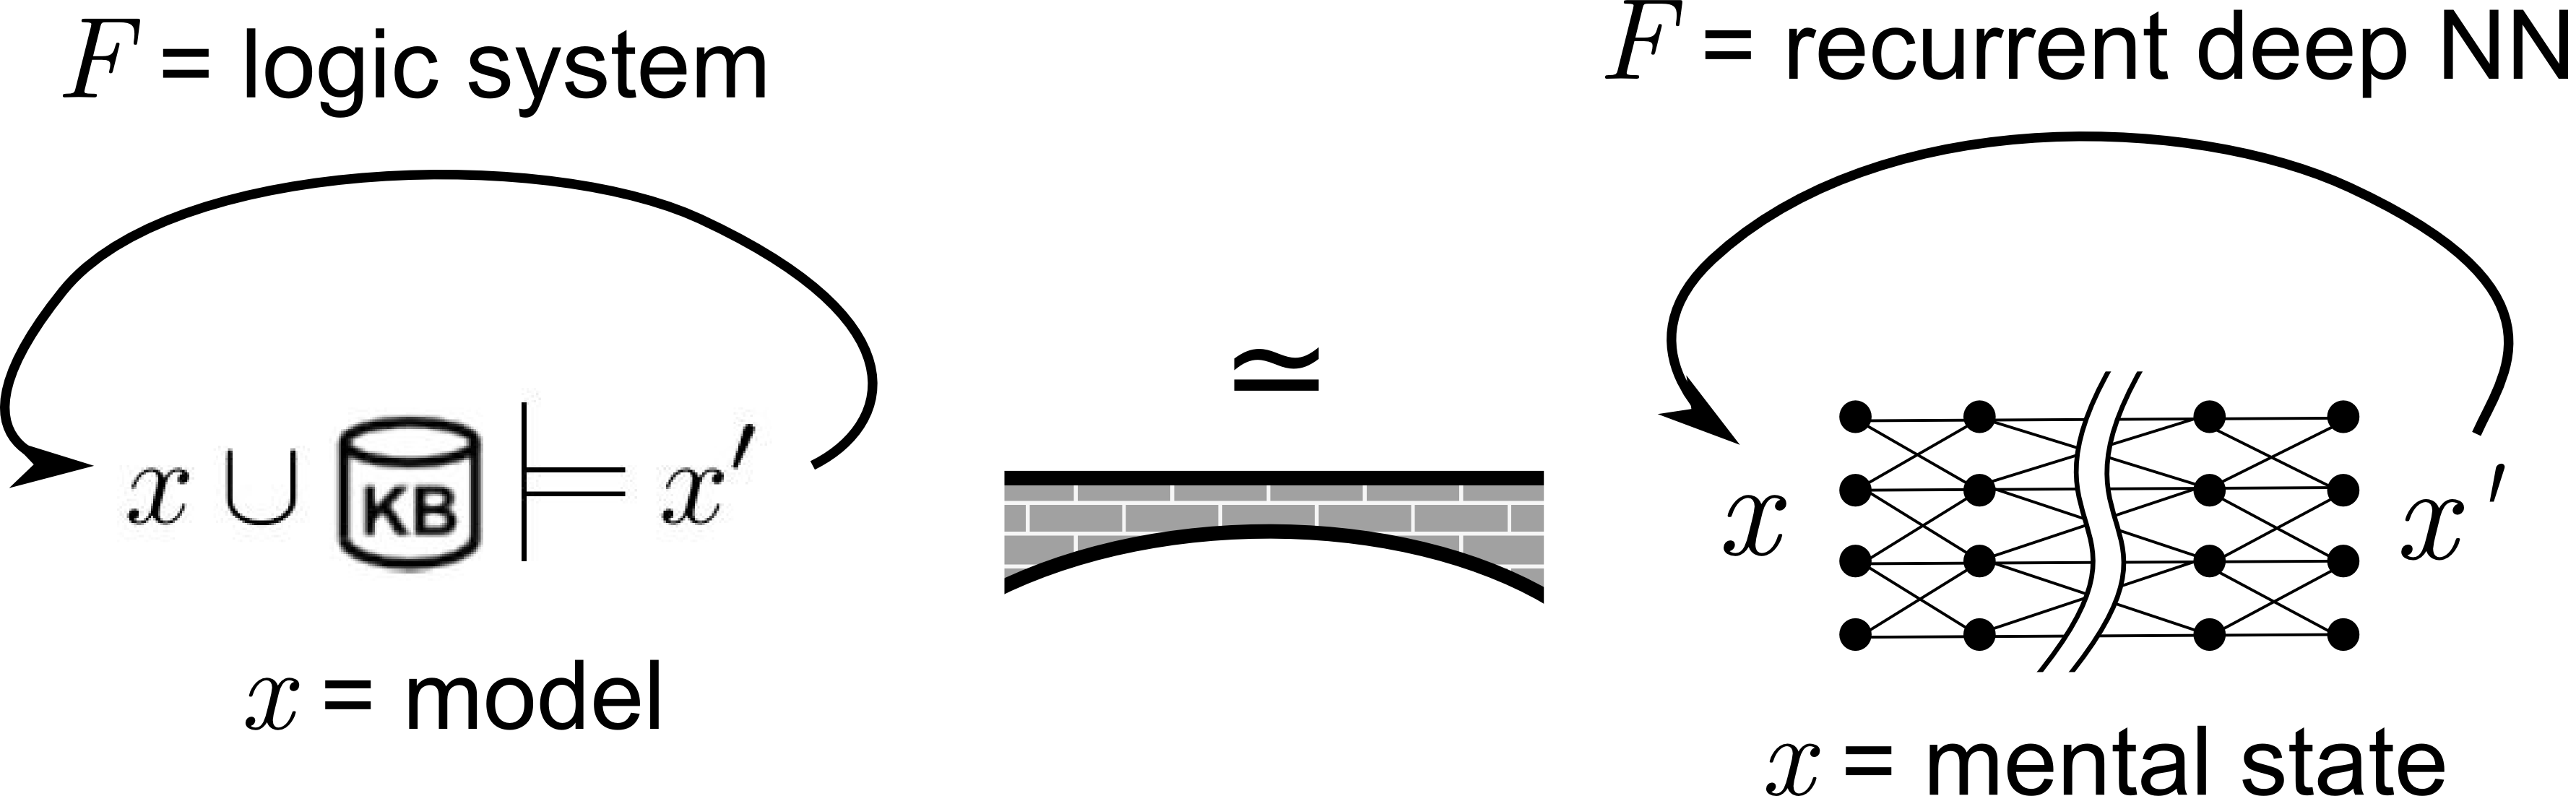
\includegraphics[scale=0.6]{bridge.png}
\end{equation}

I will first explain the structure of the logic side, and then the structure of the neural side.
%首先解释 logic 那边的结构,然后再解释 neural network 那边的结构。

% =====================================================================================
\begin{comment}

\section{Neural architecture}

Itamar Arel 在 2012 年 \cite{Arel2012}、和我在 2016 年 \cite{Yan2017}、独立地提出了同样的 cognitive architecture: 合并 \textbf{增强学习}和\textbf{深度学习}。

打个比喻来说,就是用\emp{增强学习}去控制一隻智慧生物,在「思考空间」的迷宫中找最佳路径:
\begin{equation}
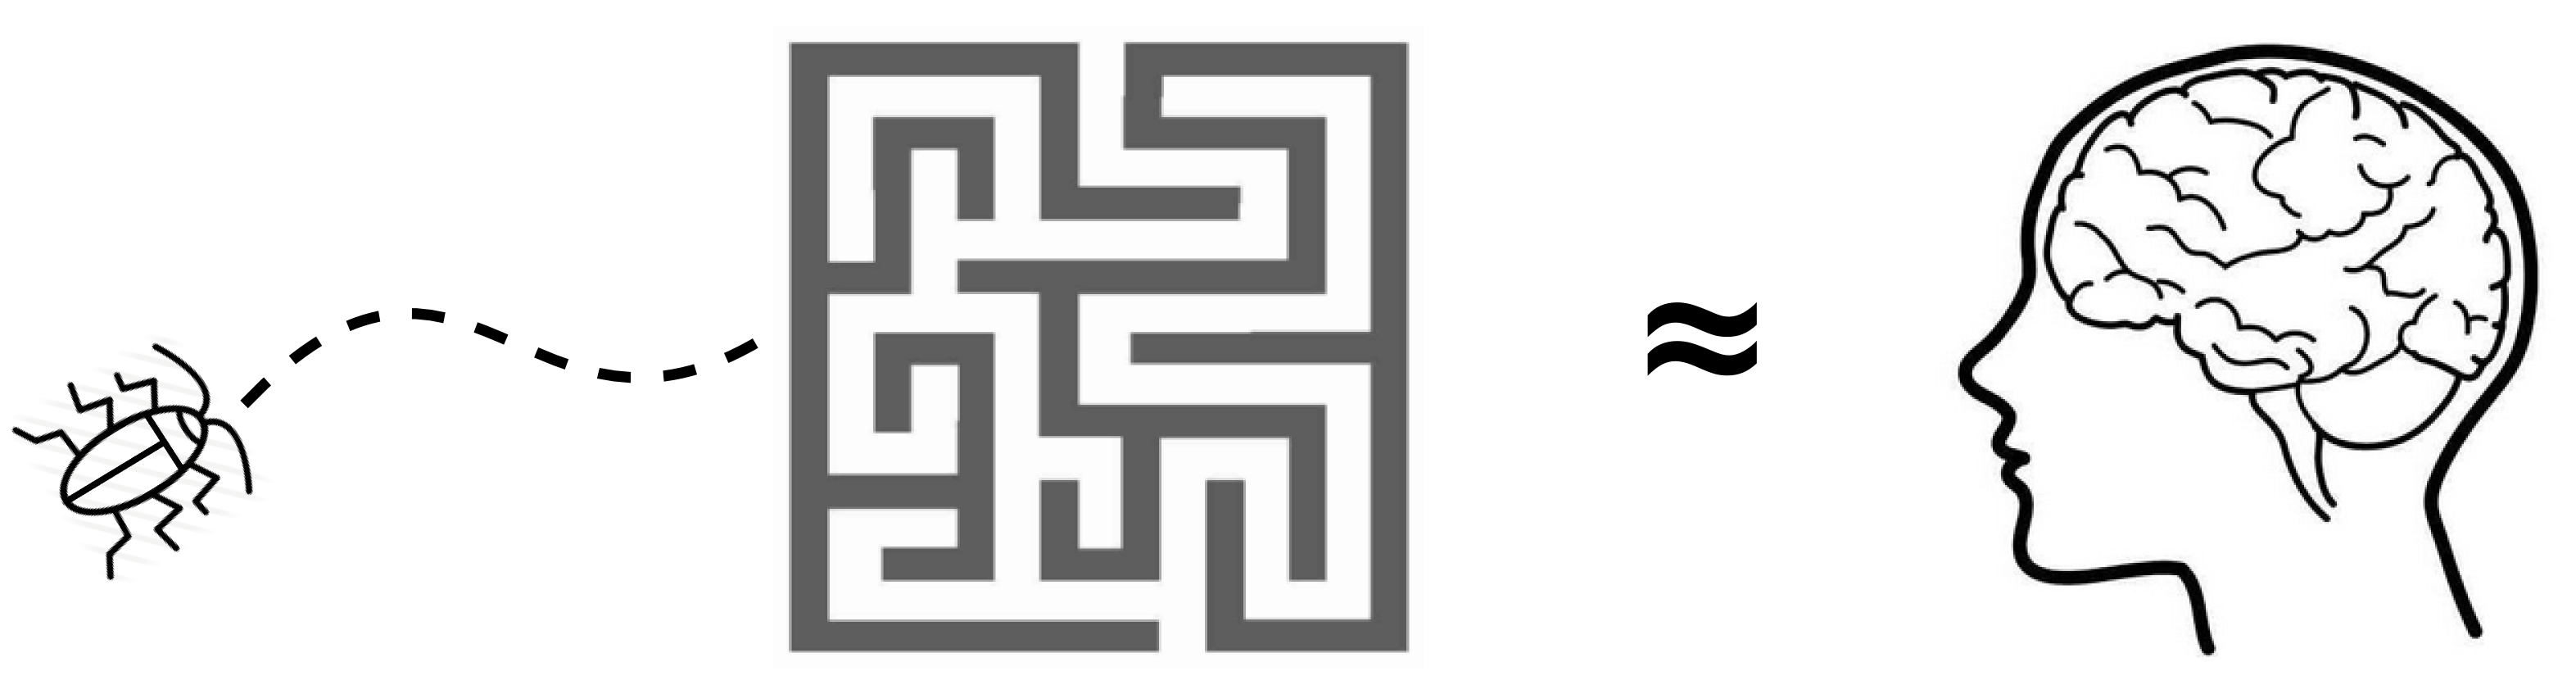
\includegraphics[scale=0.5]{maze-metaphor.png}
\end{equation}
增强学习特别适合解决这类问题,可以参看我写的 tutorial。

关键是将「思考」看成是一个\emp{动态系统} (dynamical system),它运行在\emp{思维状态} (mental states) 的空间中:
\begin{equation}
\label{fig:mental-state}
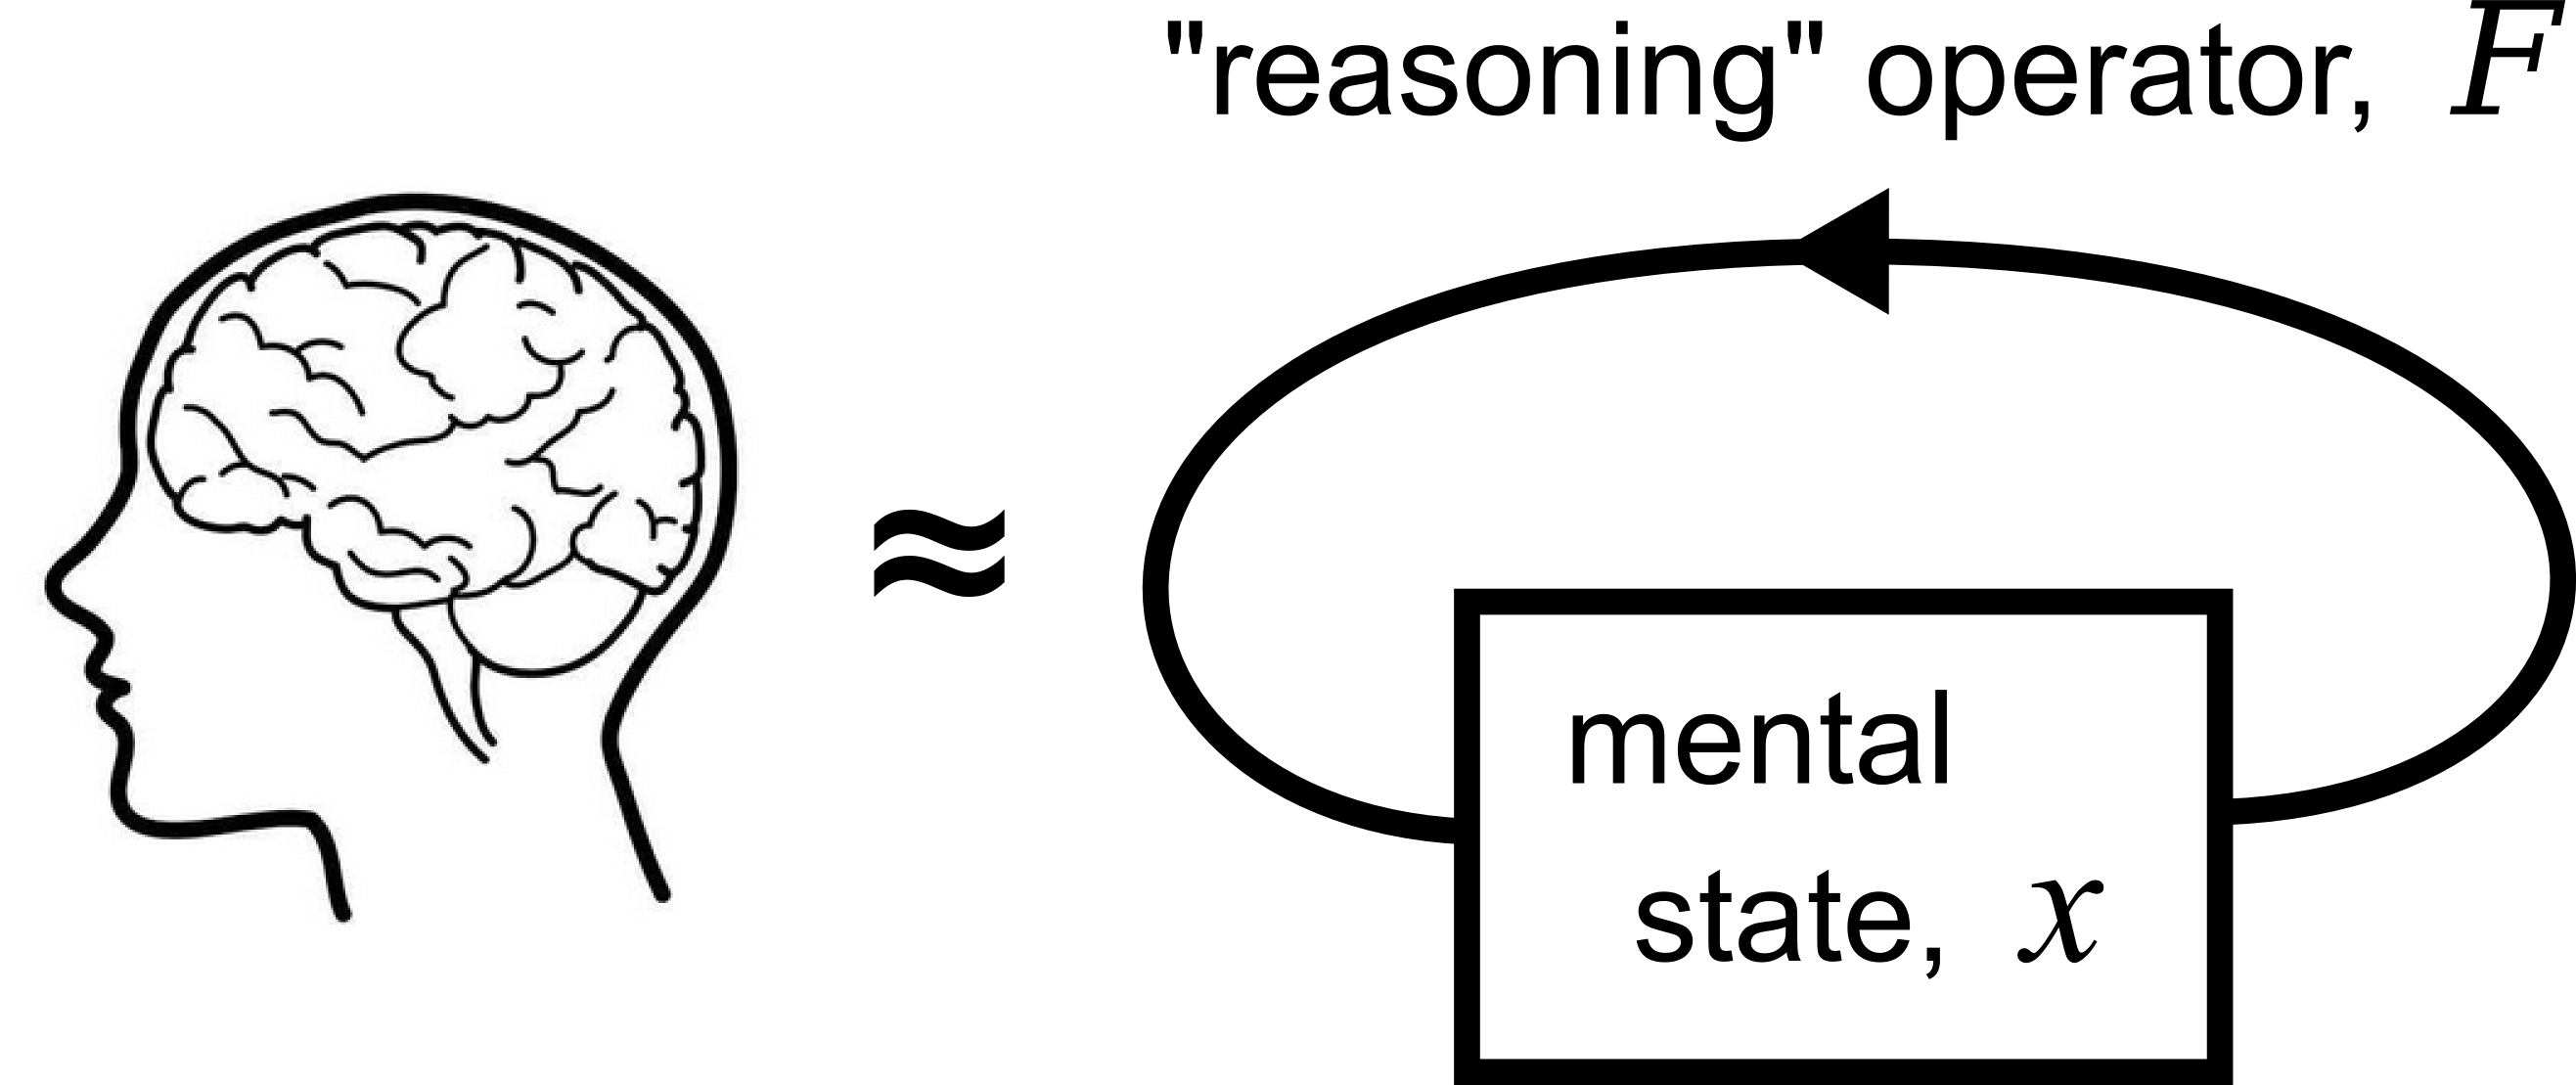
\includegraphics[scale=0.5]{mental-state.png}
\end{equation}

举例来说,一个\emp{思维状态}可以是以下的一束命题:
\renewcommand\labelitemi{\textbullet}
\begin{itemize}
\item 我在我的房间内,正在写一篇论文。
\item 我正在写一句句子的开头:「我在我的房间内,....」
\item 我将会写一个动词词组 (verb phrase):「正在写....」
\end{itemize}

思考的过程就是从一个思维状态 \emp{过渡} (transition) 到另一个思维状态。 就算我现在说话,我的脑子也是靠思维状态记住我说话说到句子结构的哪部分,所以我才能组织句子的语法。

\textbf{思维状态}是一支向量 $\vect{x} \in X$,$X$ 是全体\emp{思维空间},思考算子 (reasoning operator) $F: X \rightarrow X$ 是一个 endomorphism。

%, we would have at disposal all the tools available in vector space such as:

%\begin{itemize}
%\item numerical optimization (including gradient descent)
%\item differential equations governing time evolution
%\item dynamical systems theory, control theory (eg. adaptive filters)
%\item Lie algebra and $C^*$-algebra of continuous operators
%\item matrix theory, iteration and fixed-point theory
%\item dynamic programming (aka. reinforcement learning)
%\item neural networks and deep learning ... etc.
%\end{itemize}

% 换句话说: 我们将逻辑 AI 的整套器材搬到向量空间中去处理。 这个做法,部分是受到 Google 的 PageRank 和 Word2Vec \cite{Mikolov2013} 算法的启发,因为它们都是在向量空间中运作,而且非常成功。 %, both exploit the efficiency of vector and matrix calculus.

一个\emp{动态系统 (dynamical system)} 可以用以下方法定义:
\begin{eqnarray}
\mbox{离散时间:} \quad \quad & \vect{x}_{n+1} = \vect{F}(\vect{x}_n) \\
\mbox{连续时间:} \quad \quad & \dot{\vect{x}} = \vect{f}(\vect{x}) \label{eqn-dynsys}
\end{eqnarray}
% 其中 $f$ 也可以随时间改变。 如果 $f$ 不依赖时间,则系统是 time-invariant (定常的),形式上如(\ref{eqn-dynsys}) 那种微分方程叫作 autonomous (自主的)。
为方便起见,有时我会滥用 $F$ 和 $f$ 的表述(不区分连续和离散)。

一个(连续时间的)\emp{控制系统 (control system)} 定义为:
\begin{equation}
\dot{\vect{x}}(t) = f(\vect{x}(t), \vect{u}(t), t) \label{eqn-ctrlsys}
\end{equation}
其中 $\vect{u}(t)$ 是\emp{控制向量}。 控制论的目的就是找出最好的 $\vect{u}^*(t)$,令系统由初始状态 $\vect{x}_0$ 去到终点状态 $\vect{x_\bot}$。

% \textbf{动力系统} (\ref{eqn-dynsys}) 有标准的 Hamiltonian 力学解释,这可以看成是「思维动力学」。 系统的\textbf{相位空间}有 symplectic 结构,可以利用这结构更有效地解微分方程 (\ref{eqn-dynsys})。

% 而\textbf{控制系统} \ref{eqn-ctrlsys} 中,每次到达新状态 $x$,外部会给出一个奖励 $r(x)$,它对应於 Lagrangian,其单位是\textbf{能量}。 (换句话说,智能系统的欲望是用能量量度的; 详见 tutorial。)  

增强学习、最优控制、和 \emp{动态规划} (dynamic programming) 都是同义词。 其中心思想是 Bellman equation; 根据 Bellman update 寻找状态空间中的\emp{最优路径}。

注意: 人工智能中的 \emp{A* search},是动态规划的一个特例。 换句话说,用动态规划在某个空间中「漫游」,可以模拟 best-first 搜寻的功能。

我们的目标是学习 $F \in \{$ 无限维的算子空间 $\}$。 实践上 $F$ 可以用 deep learning network (dNN) 代表,换句话说 $F$ 就是一个有很多 parameters 的非线性算子 (= 神经网络)。 

一个\textbf{神经网络}基本上是:
\begin{equation}
F(\vect{x}) = \sigmoid(W_1 \sigmoid(W_2 ... \sigmoid(W_L \; \vect{x} )))
\end{equation}
其中 $L$ 是层数,W 是每层的权重\textbf{矩阵},$\sigmoid$ 是对每个分量的 sigmoid function (其作用是赋予非线性)。

% 所有 $W$ 的分量存在於一个\textbf{高维流形}之中,\textbf{学习}的目的就是在这流形中寻找最好的 $W^*$。 在这流形上可以定义一个\textbf{度量} (metric)(例如引入随机性之后,用 Kullback–Leibler divergence 定义),这是 information geometry 的做法,用 geodesic 可以令学习快点。 

在这框架下,智能系统的运作可以分开成两方面: \emp{思考} 和 \emp{学习}。

\emp{思考}即是根据已学得的知识(知识储存在 dNN 里),在思维空间中找寻 $\vect{x}$ 最优的轨迹,方法是用控制论计算 $\vect{u}^*$。 $\vect{x}$ 的轨迹受 dNN 约束(系统只能依据「正确」的知识去思考),但思考时 dNN 是不变的。

\emp{学习}就是学习神经网络 dNN 的 weights $W$。 此时令 $u = 0$,即忽略控制论方面。

而很明显,「自由」的 $F$ 算子没有「内部结构」,它能够学习的就像是曱甴那样的、简单的「条件反射」行为。 如果要达到人类的智慧,则要学习很久(到时我们都死了)。

所以问题就是要赋予 $F$ 更多的\textbf{结构},特别是逻辑结构。 直观地说,越多的结构令\textbf{搜寻空间}越小,学习会越快。 这是机器学习里面 inductive bias 的标准做法。

\end{comment}
% ======================================================================================

\begin{comment}
\section{Logic-based AI}

% Strong AI 的问题在理论上已经被\emp{数理逻辑}完整地描述了,馀下的问题是\emp{学习算法},因为在逻辑 AI 的架构下,学习算法很慢(复杂性很高),这就是我们要解决的。

% 我研究 logic-based AI 很多年,因此我的思路喜欢将新问题还原到逻辑 AI 那边去理解,但实际上我提倡的解决办法不是靠经典逻辑,甚至不是 symbolic 的。  但在这篇文章我还是会经常跳回到逻辑 AI 去方便理解。

用数理逻辑 (mathematical logic) 模拟人的思想是可行的,例如有 deduction, abduction, induction 等这些模式,详细可见《Computational logic and human thinking》by Robert Kowalski, 2011.  这些方面不影响本文的阅读。 值得一提的是,作者 Kowalski 是 logic programming,特别是 Prolog,的理论奠基人之一。

在经典逻辑 AI 中,「思考」是透过一些类似以下的步骤:
\begin{eqnarray}
\mbox{前提} & \vdash & \mbox{结论} \\
\boxed{\mbox{今天早上下雨}} & \vdash & \boxed{\mbox{草地是湿的}}
\end{eqnarray}
亦即由一些\emp{命题}(propositions)推导到另一些命题。

推导必须依靠一些逻辑的法则命题 (rule propositions),所谓「法则」是指命题里面带有 x 这样的\emp{变量}(variables):
\begin{equation}
\boxed{\mbox{地方 x 下雨}} \wedge \boxed{\mbox{x 是露天的}} \vdash \boxed{\mbox{地方 x 是湿的}}
\end{equation}
这些法则好比「逻辑引擎」的燃料,没有燃料引擎是不能推动的。

注意: 命题里面的 x,好比是有「洞」的命题,它可以透过 substitution 代入一些实物 (objects),而变成完整的命题。 这种「句子内部」(sub-propositional)的结构可以用 predicate logic (谓词逻辑)表达,但暂时不需要理会这些细节。

「所有人失恋了都会不开心」:
\begin{equation}
\forall z. \; \cancel\heartsuit(z) \rightarrow \frownie{}(z)
\end{equation}
在数理逻辑中这算是一条 \emp{公理} (axiom),但在 AI 中这些公理是从主体的经验中\textbf{学习}出来的,我们仍沿用「公理」这术语。 在 AI 术语中,公理的集合叫 knowledge base,记作 $\KB$。 注意 $\KB$ 是一堆 \textbf{formulas} 的集合。 

Logic-based AI 可以看成是将世界的「模型」压缩成一个 $\KB$: %,里面装著大量逻辑式子
\begin{equation}
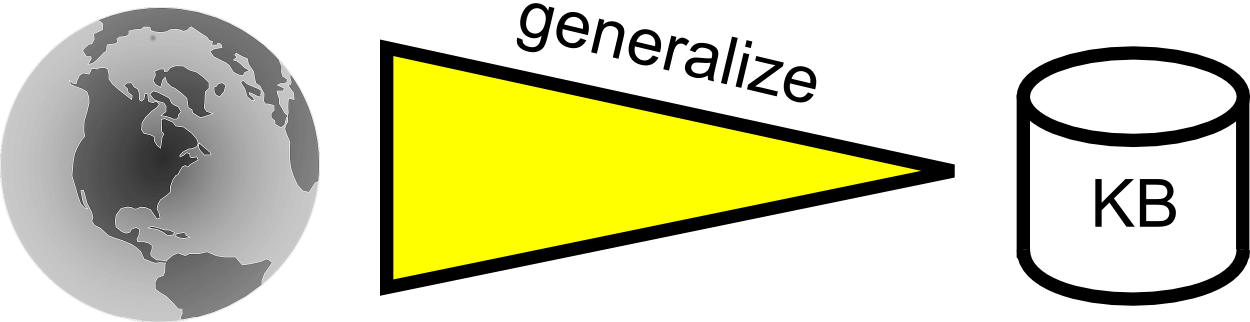
\includegraphics[scale=0.5]{world-model-compression.png}
\end{equation}
世界模型是由大量的逻辑式子经过组合而\emp{生成}的,有点像向量空间是由其「基底」生成; 但这生成过程在逻辑中特别复杂,所以符号逻辑具有很高的\emp{压缩比},但要学习一套逻辑 $\KB$,则相应地也有极高的\emp{复杂度}。

\begin{equation}
x \cup \KB \sdtstile{}{} x'
\end{equation}

\begin{equation}
\KB \, , \, \Gamma \sststile{}{} \Delta
\end{equation}

\end{comment}

\section{Structure of logic}

A \textbf{logic system} can be defined as:
\begin{itemize}
\item a set of symbols for \textbf{constants}, \textbf{predicates}, and \textbf{functions}
\item \textbf{propositions} built from the above atoms
\item \textbf{connectives} between simple propositions, eg:  $\neg, \wedge, \vee$
\item The \textbf{logical consequence} relation: $\Gamma \vdash \Delta$
% \item 命题的内部结构(命题由概念原子组合而成)
\end{itemize}

Personally I think \textbf{relation algebra} \cite{Schmidt2010} \cite{Maddux2006} is closer to human natural language, but the standard form used in mathematical logic research is first-order logic (FOL).  This is however not of the essence, because all logics are basically easily interconvertable.  In the following we concentrate on FOL.
%个人认为 relation algebra \cite{Schmidt2010} \cite{Maddux2006} 比较接近人类自然语言,但在数理逻辑研究中最通用的逻辑是 first-order logic (FOL)。 然而这并不是重点,因为各种逻辑基本上是等效的,而且相互之间可以很容易地转换。 以下集中讨论 FOL。  

From raw sensory data, we can \textbf{inductively} learn a set of logic formulas, ie. the knowledge base $\KB$.  This process is under the research heading of \textbf{inductive logic programming} (ILP).  Everyone familiar with classical AI knows ILP, but in recent decades the popular focus is on \textbf{statistical learning}, and this kind of symbolic logic learning is relatively neglected.
%由一些原始的 sensory data,可以透过逻辑学习出一些 logic formulas,即知识库 (knowledge base) $\KB$。 这个过程叫逻辑\textbf{诱导学习} (inductive logic programming, ILP)。 学经典 AI 的人都知道 ILP,但近数十年来,注意力集中在统计学习,这种符号逻辑的学习法被忽视。 

Raw sensory data can be processed using neural-based pattern recognition, or it can be processed via ILP-based pattern recognition.  The result of these two pathways should obviously be isomorphic (at least approximately):
\begin{equation}
\begin{tikzcd}[]
\mbox{Logic representation} \arrow[rr, phantom, "\simeq"] & & \mbox{Neural representation} \\
& \arrow[ul, "\mbox{inductive logic learning}"] \arrow[ur, "\mbox{deep NN learning}" swap] 
\includegraphics[scale=0.5]{sensory-data.png} &
\end{tikzcd}
\end{equation}

I have spent a lot of time thinking how to transition logic-based representations to the neural side, but found this target to be very elusive.
%我以前花了很多时间思考怎样将逻辑的 representation 过渡到神经网络去,但发觉这个目标非常 elusive。

On the one hand, logic is the study of the laws of human thinking, developed over centuries.  The logical description is correct;  There should be a correspondence between logic and neural, as they are both doing the same thing (intelligence).
%一方面,逻辑是几百年来发展起来的关於人类思考的规律; 逻辑的描述是正确的; 逻辑和神经之间必然有一个 correspondence,因为它们都在做同样的事(智能)。 

In \textbf{cognitive science}, many researchers believe the representations inside our brains are so-called ``mental models'', and few would believe that the brain uses a representation like the propositions in symbolic logic, or to think with the sort of symbolic manipulations as $\lambda$-calculus.
%在\textbf{认知科学}里,有很多人相信大脑的内部的 representation 是一些所谓 ``mental models'',而很少人会相信大脑使用一些像命题那样的符号结构做 representation,甚至用 $\lambda$-calculus 那样的符号 manipulation 去思考。

As an example, when we verbally describe a case of murder, the reader would establish in her mind's eye a ``model'' that is similar to real experience yet is unreal.  The human brain seems to use such mental models to think, rather than with a bunch of propositions.  Examples of model-based reasoning using logic are \cite{Magnani1999} \cite{Magnani2002}.
%举例来说,用文字描述一起凶杀案,读者心目中会建立一个「模型」,它类似於真实经验但又不是真实的。 人脑似乎是用这样的 mental models 思考,而不是一些命题的集合。 %至於 mental models 是什么,目前认知科学还未有定论。

So eventually I realized that the logic-neural correspondence must be achieved through model theory:
\begin{equation}
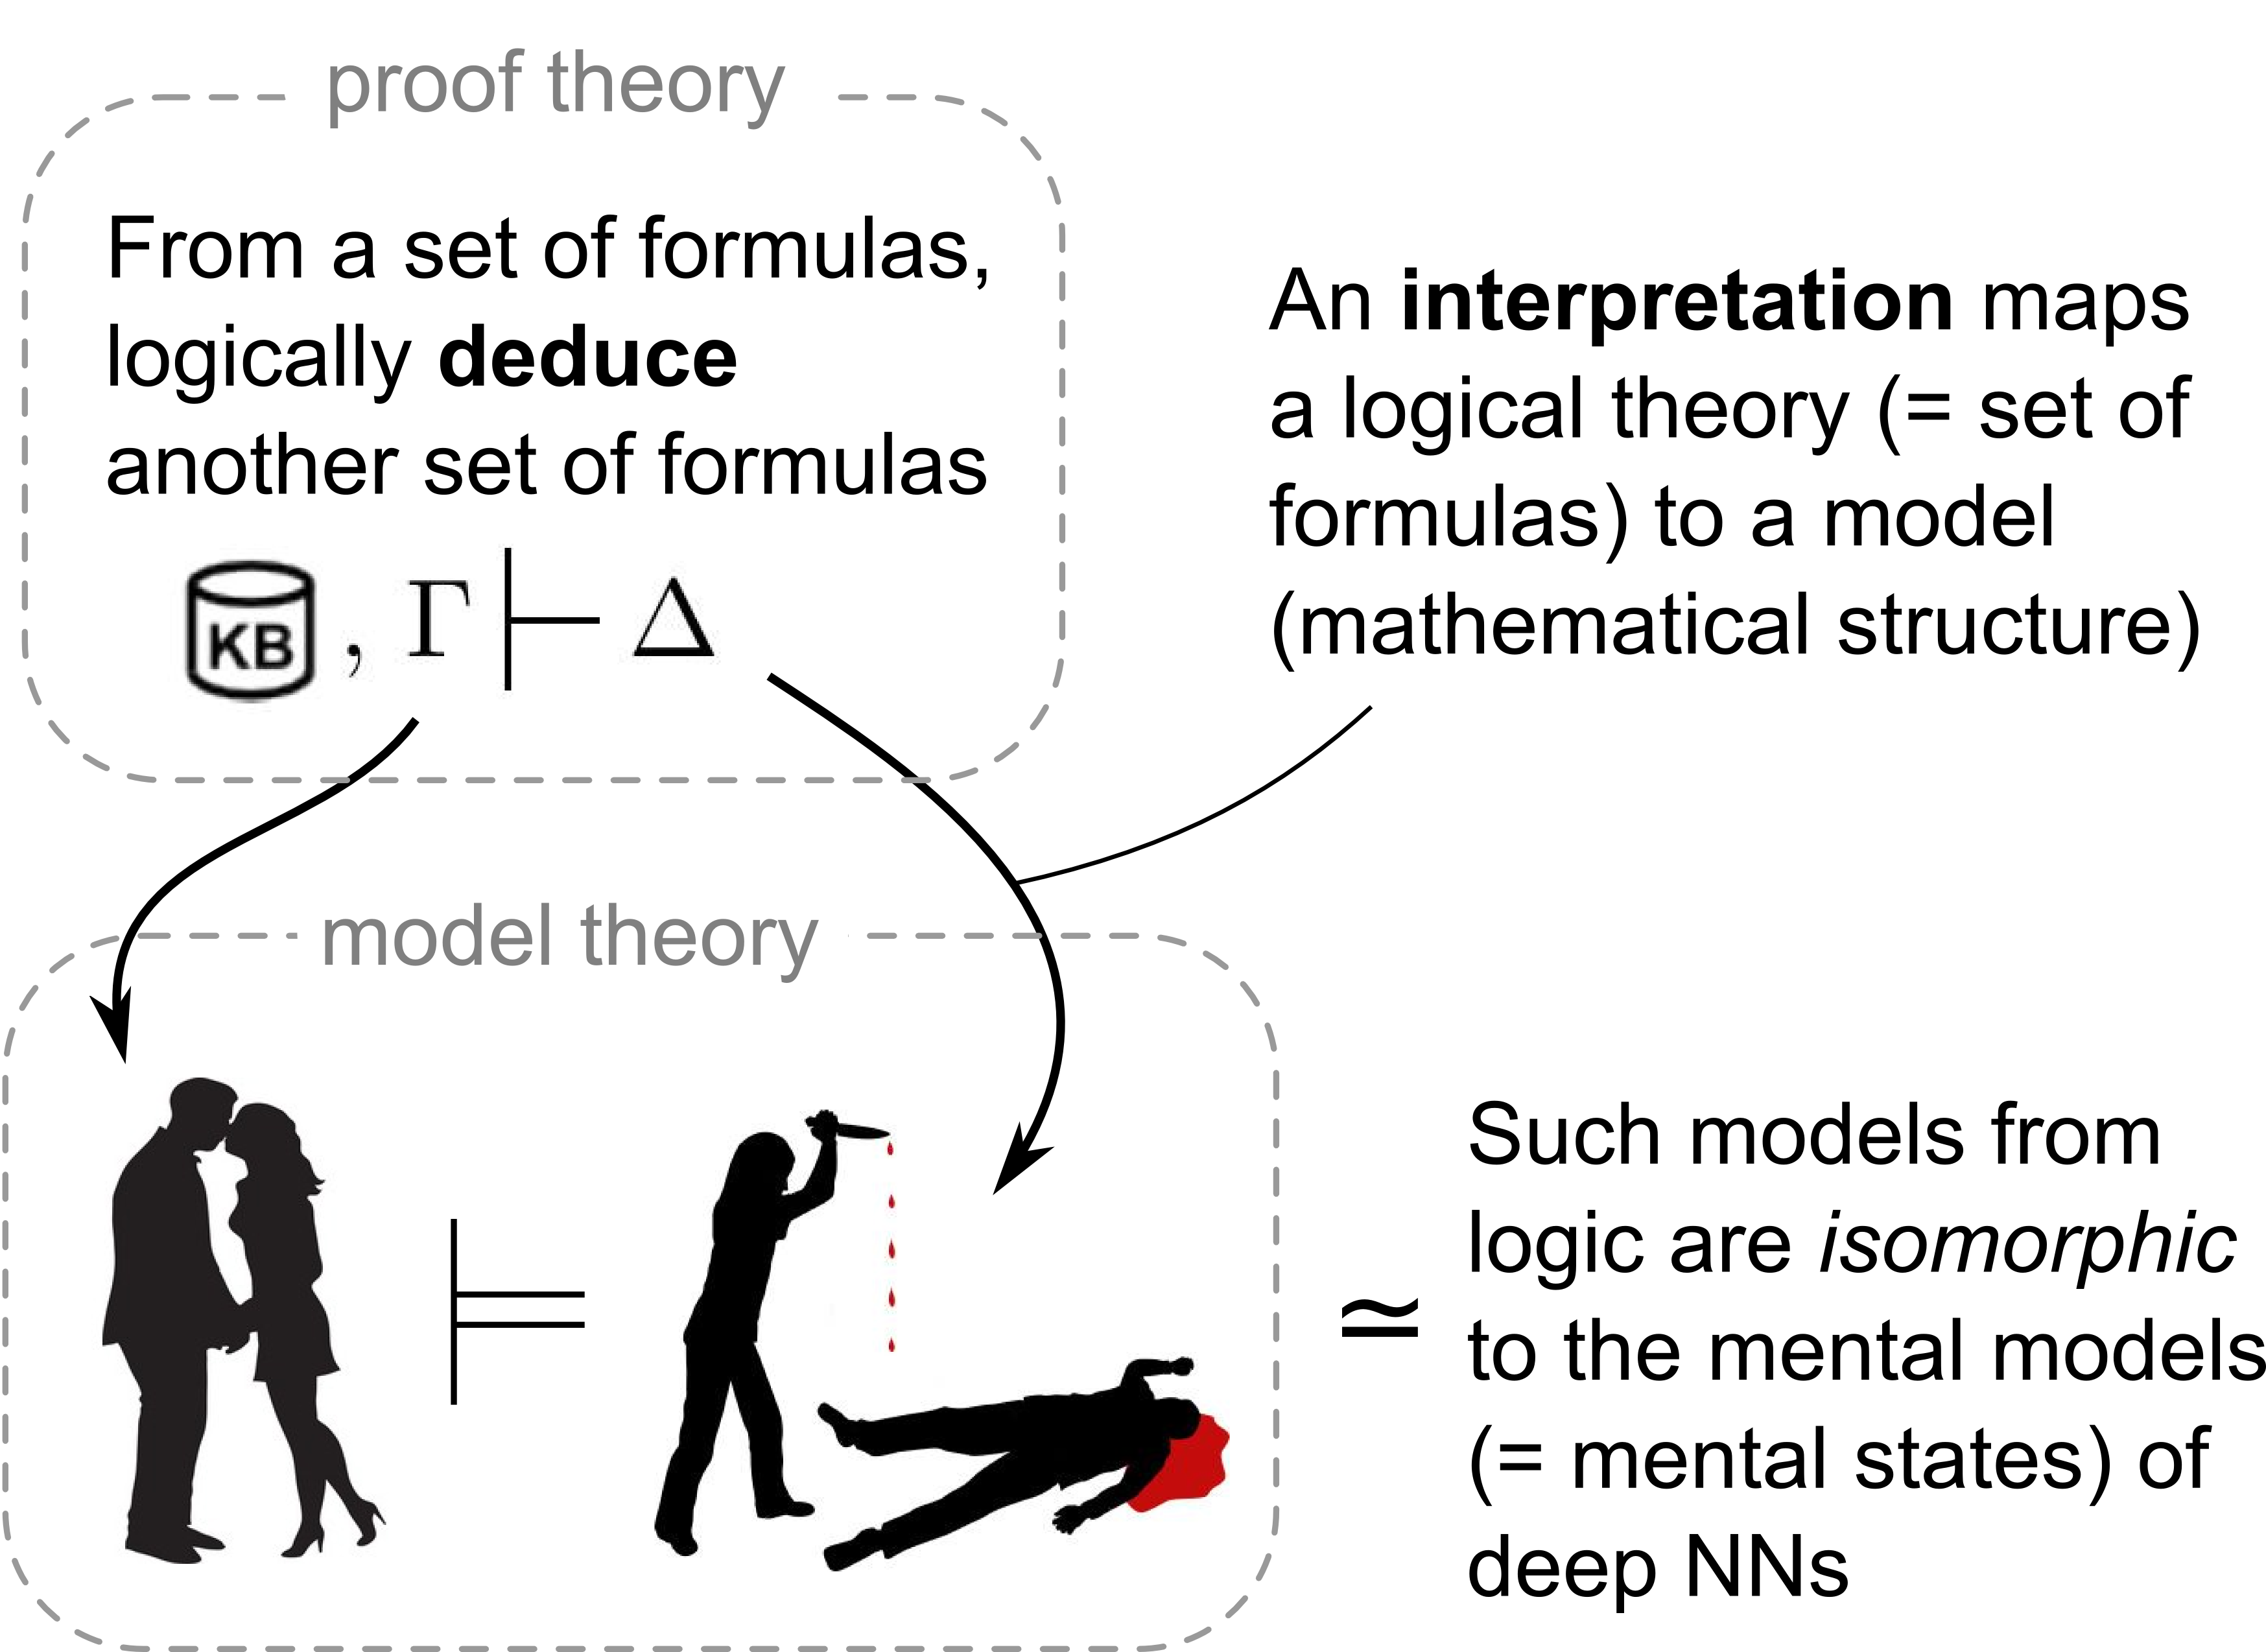
\includegraphics[scale=0.75]{model-theory.png}
\end{equation}

$\vdash$ means deducing from a set of (symbolic logic) \textbf{formulas} to new formulas.  $\vDash$ means that a \textbf{model} necessarily entails another model.

% \footnote{Knowledge-based model construction (\textbf{KBMC}) 这个术语较少人知道,但其实是最关键的结构; 换句话说,就是从 $\KB$ 中抽出一组命题 $\Gamma$,去\textbf{组合}一个 model 或 proof tree,而这个 proof tree 的某个节点,就是新的结论。 亦即 $\Gamma \vdash Q$。 KBMC 的概念适用於经典逻辑也适用於 Bayesian networks。}

% ====================================================================================
\begin{comment}
\subsection{由一些命题推导出另一些命题}

命题也有内部结构(即命题可以由概念原子组合而成),但我们先从最简单情况谈起,即\textbf{命题逻辑}。

最简单的经典命题逻辑,是 Boolean propositional logic,它的\textbf{代数形式}是我们熟悉的 Boolean algebra,二者几乎没有分别(纯粹逻辑符号和代数符号的对应)。 

在 Boolean algebra 可以定义一种 ideal $I$:
\begin{itemize}
\item If $a, b \in I$ then $a \wedge b \in I$
\item If $a \in I$ and $a \le b$ then $b \in I$
\end{itemize}
其中 $a \le b$ 表示 $a \Rightarrow b$(a 蕴涵 b)。

由上面可以看出,这个 ideal 其实是由某些元素(命题)生成的 \textbf{逻辑后果}(logical consequence); 换句话说,给定一个命题集 $\Gamma$,问 $\Gamma \stackrel{?}{\vdash} a$(从 $\Gamma$ 可以推导出 $a$ 吗?) 就等於问 $a$ 是不是 $\Gamma$ 生成的 ideal membership 问题。 也可以说,代数 ideal $\equiv$ 逻辑 consequence。 (严格来说,consequence 对应的是 filter 的概念,而 filter 是 ideal 的 dual,因为 0 和 1 对应的倒错,但这不是重点。)

\textbf{逻辑后果}可以记作 $\vdash$ 或 Cn,Tarski 定义了 $\vdash$ (很明显)的特性:
\begin{itemize}
\item (reflexivity): \quad $A \vdash A$ for every formula $A$
\item (monotonicity): \quad $A \vdash Q$ implies $A, B \vdash Q$
\item (`cut'): \quad \quad $A \vdash B$ and $A, B \vdash Q$ implies $A \vdash Q$
\end{itemize}

% 在 Boolean algebra 中有一些 inference rules,例如:

以上是 Boolean logic 的代数化,但如果考虑 probabilistic logic 就更为复杂,需要用到 Bayesian networks,而 filter $\equiv$ consequence 的原理似乎不再适用。 

Bayesian network 的细节很麻烦,可以花整个研究生课程来讲。

重点是: Bayesian network 是由一些\textbf{条件概率} (conditional probability) 的关系生成的。 每个\textbf{节点}是一个命题,每个\textbf{连结}是一个条件概率关系,例如:
\begin{equation}
P(A|B,C,D,...) = \vec{p}
\end{equation}
其中 $\vec{p}$ 是一个 conditional probability table (CPT)。

对不起,用一个较粗俗的例子说明(在我多年的教学经验里,这是最易懂的例子):
\begin{equation}
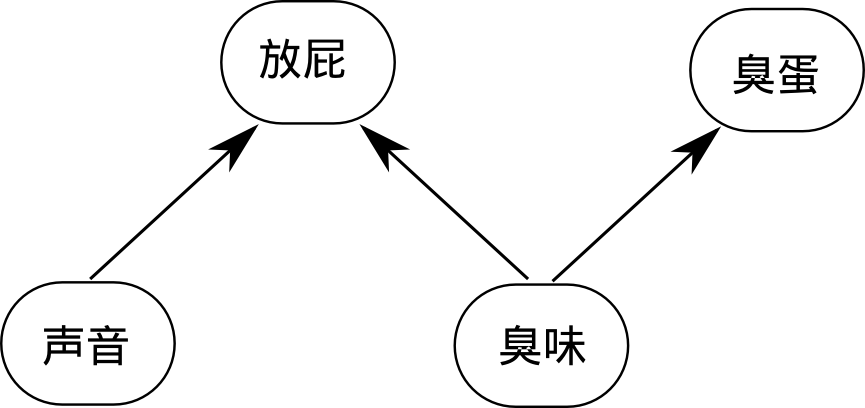
\includegraphics[scale=0.5]{farting.png}
\end{equation}
这个 Bayesian network 是由两个 CPT 生成的:
\begin{eqnarray}
P(\mbox{放屁} | \mbox{臭味}, \mbox{声音}) = \vec{p}_1 \nonumber \\
P(\mbox{臭蛋} | \mbox{臭味}) = \vec{p}_2
\end{eqnarray}
如果有「声音」又有「臭味」,则「有人放屁」的机率很高,而「臭蛋」的机率却会减少。 换句话说,「臭蛋」的机率被扯到「放屁」那边去了; 这个现象叫 ``explaining away'',它说明 Bayesian network 中,所有节点都是 globally 相关的。 所以,当求解 Bayesian network 的某个节点时,它的概率会是一连串很复杂的 sum-product 形式。 看来用 Bayesian network 表示 $\vdash$ 的方法太复杂了。

可幸的是,可以用 Monte Carlo 方法求解 Bayesian network: 开始时随机地指定节点的概率,然后随机地选取某些节点来作「\textbf{局部}」的 update; 当随机 update 的次数趋近无限,节点的机率会收敛到正确的值。 换句话说: 这是一个 \textit{local} 的计算 Bayesian network 的方法。

% ==================================================================================
\end{comment}

\section{Model theory}

For the basics of model theory, cf \cite{Doets1996} \cite{Manzano1999}.  The model-theoretic approach is to separate the \textbf{symbolic language} $\mathcal{L}$ and the $\mathcal{L}$-structures it refers to.  They are related by \textbf{interpretation} maps.

% 模型论基础可参看 \cite{Doets1996} \cite{Manzano1999}。 模型论的做法是将逻辑的符号\textbf{语言} (language $\mathcal{L}$) 和它所指涉的\textbf{结构} $\mathcal{L}$-structure 分割,中间用 interpretation map 关联起来。

$\mathcal{L}$ contains the set of symbols (predicates, relations, functions, constants), which recursively generates formulas and compound formulas.  These are the \textbf{symbolic} stuff.

%$\mathcal{L}$ 就是符号的集合 (predicates, relations, functions, constants),递归地生成出句子和复合句子。 这些都是 symbolic 的东西。

An $\mathcal{L}$-structure can be any abstract algebraic structure.  It usually consists of a \textbf{base set}, and functions and relations defined over that set.

%$\mathcal{L}$-structure 可以是任何抽象代数结构,它通常包含一个 base 集合,然后在集合上定义一些函数和关系。 

The central idea of model theory is using the interpretation map $i$ to ``preserve'' certain relations, for example:

%模型论的中心思想是透过 interpretation $i$ 去「保存」一些关系,例如:
\begin{equation}
R(a,b) \stackrel{i}{\mapsto} R^\mathcal{M}(a^\mathcal{M}, b^\mathcal{M})
\end{equation}

$R$ is a relation, $x^\mathcal{M}$ denotes the object corresponding to $x$ in the structure $\mathcal{M}$.  The left side is symbolic logic;  the right side is the actual structure.  When model theory is applied to first-order logic, we get the equivalence of $\vdash$ and $\vDash$ (which looks like tautology).  This can be found in any mathematical logic textbook, such as \cite{Hedman2004}.

%$R$ 是一个关系,$x^\mathcal{M}$ 代表在结构 $\mathcal{M}$ 之上,$x$ 所对应的物体。 左边是符号逻辑,右边是实体的结构。 模型论应用在 first-order logic,得出 $\vdash$ 和 $\vDash$ 等价的结论(看起来就好像同语反覆),这在数理逻辑教科书中都有,例如 \cite{Hedman2004}。 

If we use category theory to express the correspondence between logic and neural:
%如果用範畴论的方法表示逻辑结构和神经结构之间的对应:
\begin{equation}
\begin{tikzcd}[]
\mathcal{L} \arrow[d, "i"] \\
\mathcal{M} \arrow[r, phantom, "\simeq"] & \mathcal{X} \\
& \arrow[u, "\mbox{deep NN}" swap] \mathcal{S}
\end{tikzcd}
\end{equation}
\begin{itemize}
\item $\mathcal{L}$ = category of logic theories (= sets of formulas)
\item $i$ = interpretation maps
\item $\mathcal{M}$ = category of models (from logic)
\item $\mathcal{X}$ = category of models (from deep NNs)
\item $\mathcal{S}$ = sensory input
\end{itemize}

The above diagram says the same as this cartoon explanation:
%上图等同於下面的卡通解释:
\begin{equation}
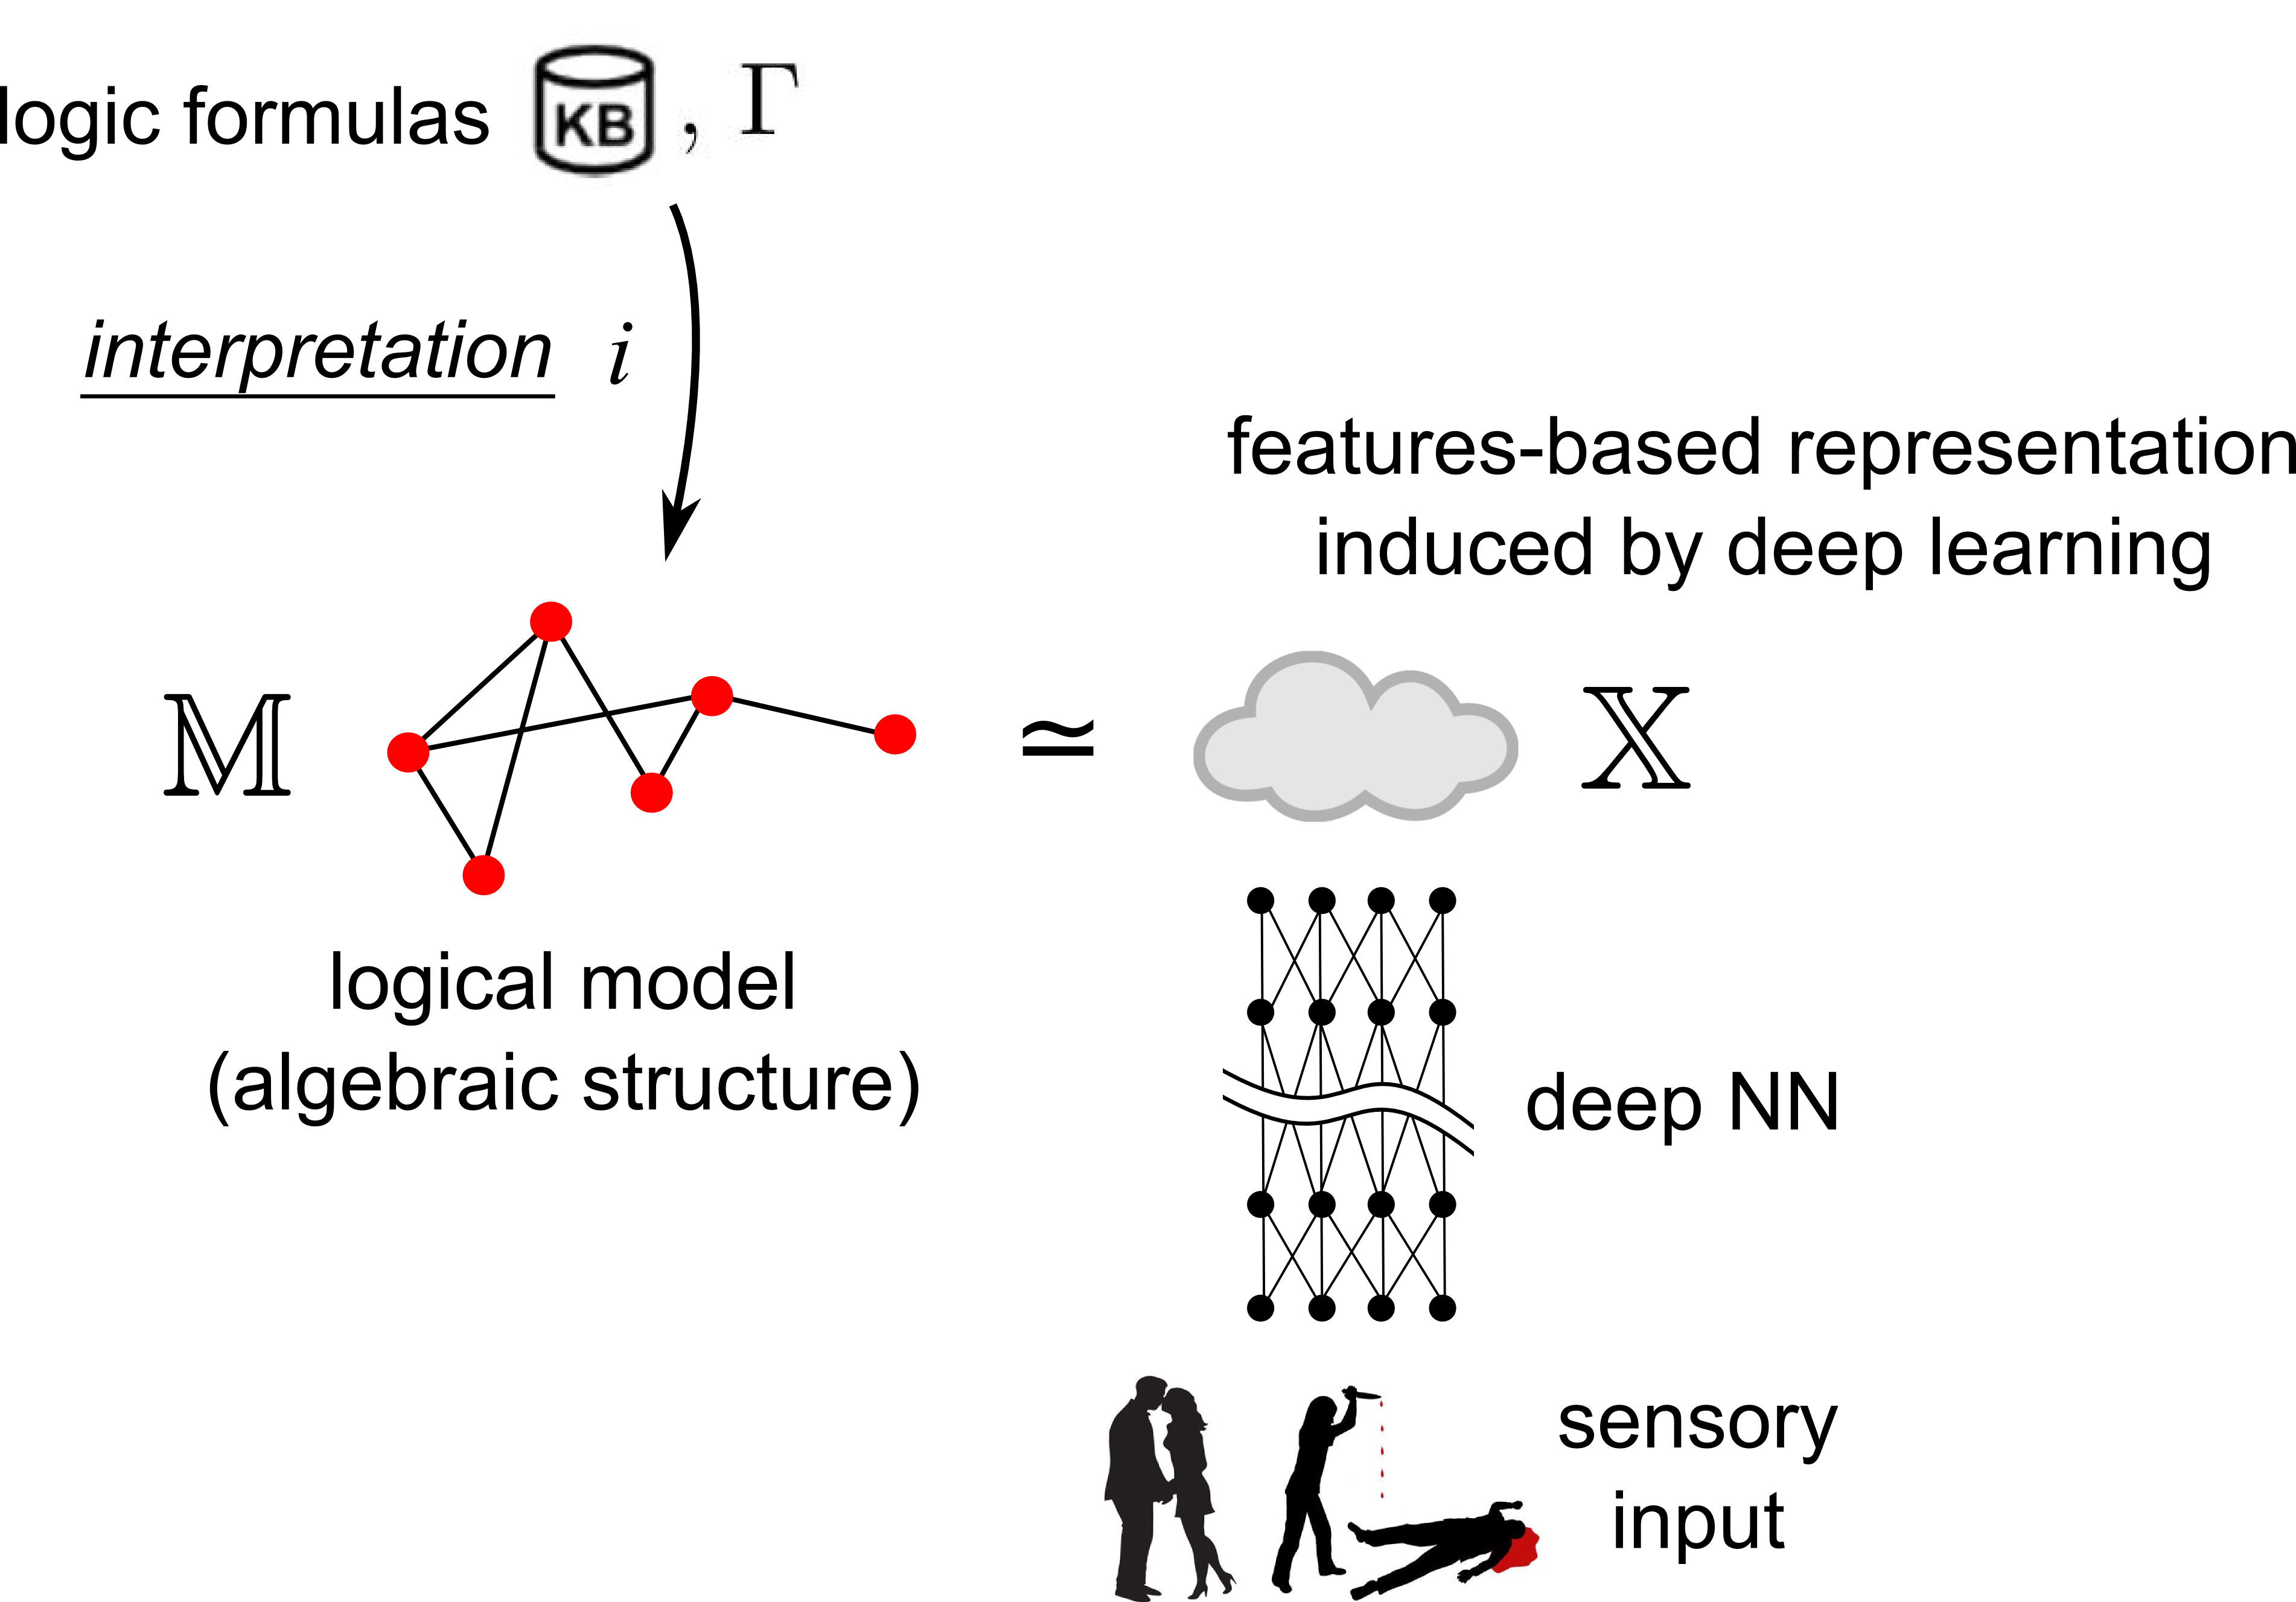
\includegraphics[scale=0.7]{model-theory-cartoon.png}
\end{equation}

In other words, $\mathcal{X} = \vcenter{\hbox{
\includegraphics{cloud.png}}}$ is \textbf{induced} from deep learning;  but its structure is \textbf{opaque} to us (that is the weakness of neural networks).
%换句话说,$\mathcal{X} = \vcenter{\hbox{
\includegraphics{cloud.png}}}$ 是由深度学习 induce 出来的结构; 但它的结构对我们来说是不透明的(这是神经网络的弱点)。

Whereas, the structure of $\mathcal{M} = \vcenter{\hbox{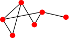
\includegraphics{algebraic-model.png}}}$ is the subject matter of model theory.

%而 $\mathcal{M} = \vcenter{\hbox{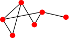
\includegraphics{algebraic-model.png}}}$ 的结构就是模型论研究的对象。
%是 free 的; 换句话说,那 $i$ map 的 source domain 是固定的,但 target domain 是自由的。 这导致 $i$ map 的学习很困难,因为 $\mathcal{M}$ 和 $\mathcal{X}$ 的结构都不清楚。 必须更详细分析 $\mathcal{M}, \mathcal{X}$ 的结构。

%\section{模型论和 interpretation 的结构}

In model theory, $\mathcal{L}$ is the category of logic formulas, $\mathcal{M} = \vcenter{\hbox{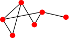
\includegraphics{algebraic-model.png}}}$ could be any algebraic structure.  We just need to map the constants, predicates, relations, functions in $\mathcal{L}$ to the structure in $\mathcal{M}$.  For the sake of conciseness, we will just constants symbols and relation symbols, as these two are the \textbf{essence} of logic.

%在模型论中,$\mathcal{L}$ 是逻辑句子的範畴,$\mathcal{M} = \vcenter{\hbox{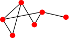
\includegraphics{algebraic-model.png}}}$ 可以是任何抽象代数结构。 只需把 $\mathcal{L}$ 中的 constants, predicates, relations, functions 映射到 $\mathcal{M}$ 就行。 为简化讨论,我们只考虑 constants 和 relations,因为二者是逻辑中最\textbf{本质}的东西。 
\begin{eqnarray}
\mathcal{L} & \quad \stackrel{i}{\rightarrow} \quad & \mathcal{M} \nonumber \\
\mbox{constant symbol} & \quad \stackrel{i}{\mapsto} \quad & \; 
\includegraphics[scale=0.5]{node.png} \\
\mbox{relation symbol} & \quad \stackrel{i}{\mapsto} \quad & \; 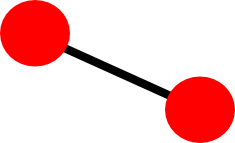
\includegraphics[scale=0.5]{link.png} \nonumber
\end{eqnarray}

Our problem is that we don't know the structure of  $\vcenter{\hbox{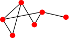
\includegraphics{algebraic-model.png}}}$.  For a long time, researchers have treated neural networks as ``black boxes'', but if we don't know the structure of $\mathcal{X} =  \vcenter{\hbox{
\includegraphics{cloud.png}}}$ we cannot build the isomorphism $\mathcal{M} \simeq \mathcal{X}$.

%问题是在神经那边缺乏 $\vcenter{\hbox{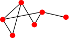
\includegraphics{algebraic-model.png}}}$ 的结构。 一直以来,人们习惯把神经网络看成是 ``black box'',但如果我们不知道 $\mathcal{X} =  \vcenter{\hbox{
\includegraphics{cloud.png}}}$ 的结构,就无法建立 $\mathcal{M} \simeq \mathcal{X}$ 的 isomorphism。

\section{The structure of neural networks}

So, what is the structure of neural network representations?
%那么,神经网络的 representation 究竟是什么结构?  

Basically a \textbf{neural network} is:
%一个\textbf{神经网络}基本上是:
\begin{equation}
F(\vect{x}) = \sigmoid(W_1 \sigmoid(W_2 ... \sigmoid(W_L \; \vect{x} )))
\end{equation}
where $L$ is the number of layers, $W_\ell$ is the \textbf{weight matrix} for each layer, $\sigmoid$ is the sigmoid function applied component-wise to each neuron (whose role is to provide \textbf{non-linearity}).

%其中 $L$ 是层数,$W_\ell$ 是每层的权重\textbf{矩阵},$\sigmoid$ 是对每个分量的 sigmoid function (其作用是赋予非线性)。

$\sigmoid$ acts on each component of $\vect{x}$;  Its action is \textbf{not invariant} under a change of coordinates.  Therefore, $\sigmoid$ is not a vector operation, and thus \ul{$\mathcal{X}$ is also not a \textbf{vector space} structure}.  Common practice is to denote $\vec{x}$ as a vector, but this is misleading.
%$\sigmoid$ 作用在 $\vect{x}$ 的每个分量上,它的作用在座标变换下\textbf{没有不变性}。 所以 $\sigmoid$ 不是一个向量运算,从而 \underline{$\mathcal{X}$ 的结构也不是\textbf{向量空间}的结构}。 通常习惯把 $\vec{x}$ 写成向量形式,但这是误导的。

If we connect a neural network \textbf{head to tail} forming a loop, we get the simplest form of a cognitive architecture, whose \textbf{state equation} is $\vect{x}_{n+1} = F(\vect{x}_n)$, or in continuous time $\dot{\vect{x}} = f(\vect{x})$.  From this we can see that $\vect{x} \in \mathcal{X}$ is a \textbf{differential manifold}.  The deeper theory is that it is a Hamiltonian system, having the \textbf{symplectic} structure. In other words, $\mathcal{X}$ is a differential manifold endowed with a symplectic metric.  But this is outside the scope of this paper, please refer to my \cite{Yan2017}.

%如果将神经网络\textbf{首尾相接}造成迴路,这是一种智能系统的最简单形式,它的状态方程是 $\vect{x}_{n+1} = F(\vect{x}_n)$ (或连续时间的 $\dot{\vect{x}} = f(\vect{x})$),由此可以看出,$\vect{x} \in \mathcal{X}$ 是一个\textbf{微分流形}。 更深入地讲,它是一个力学上的 Hamiltonian 系统,具有 symplectic(辛流形)结构。 换句话说,它是微分流形,而且有一个辛度量 (metric)。 但这超出了本文範围,详见作者的 \cite{Yan2017}。

% 所以问题就是要赋予 $F$ 更多的\textbf{结构},特别是逻辑结构。 直观地说,越多的结构令\textbf{搜寻空间}越小,学习会越快。 这是机器学习里面 inductive bias 的标准做法。

Now let's think about how a neural network performs pattern recognition, perhaps it would be illuminating:
%现在思考一下,神经网络怎样识别模式,或许会有帮助:

Consider the simplest case, eg. a layer of neural network extracting visual features from the digit ``9''.  This layer may have many neurons (left figure), each neuron locally covers a region of the input layer, the so-called ``local receptive field'' in the neuroscience of vision (right figure).
%考虑最简单的情况,例如提取 digit ``9'' 的特徵的一层网络。 这层网络可以有很多神经元(左图),每个神经元局部地覆盖输入层,即所谓视觉神经元的 local receptive field(右图)。
\begin{equation}
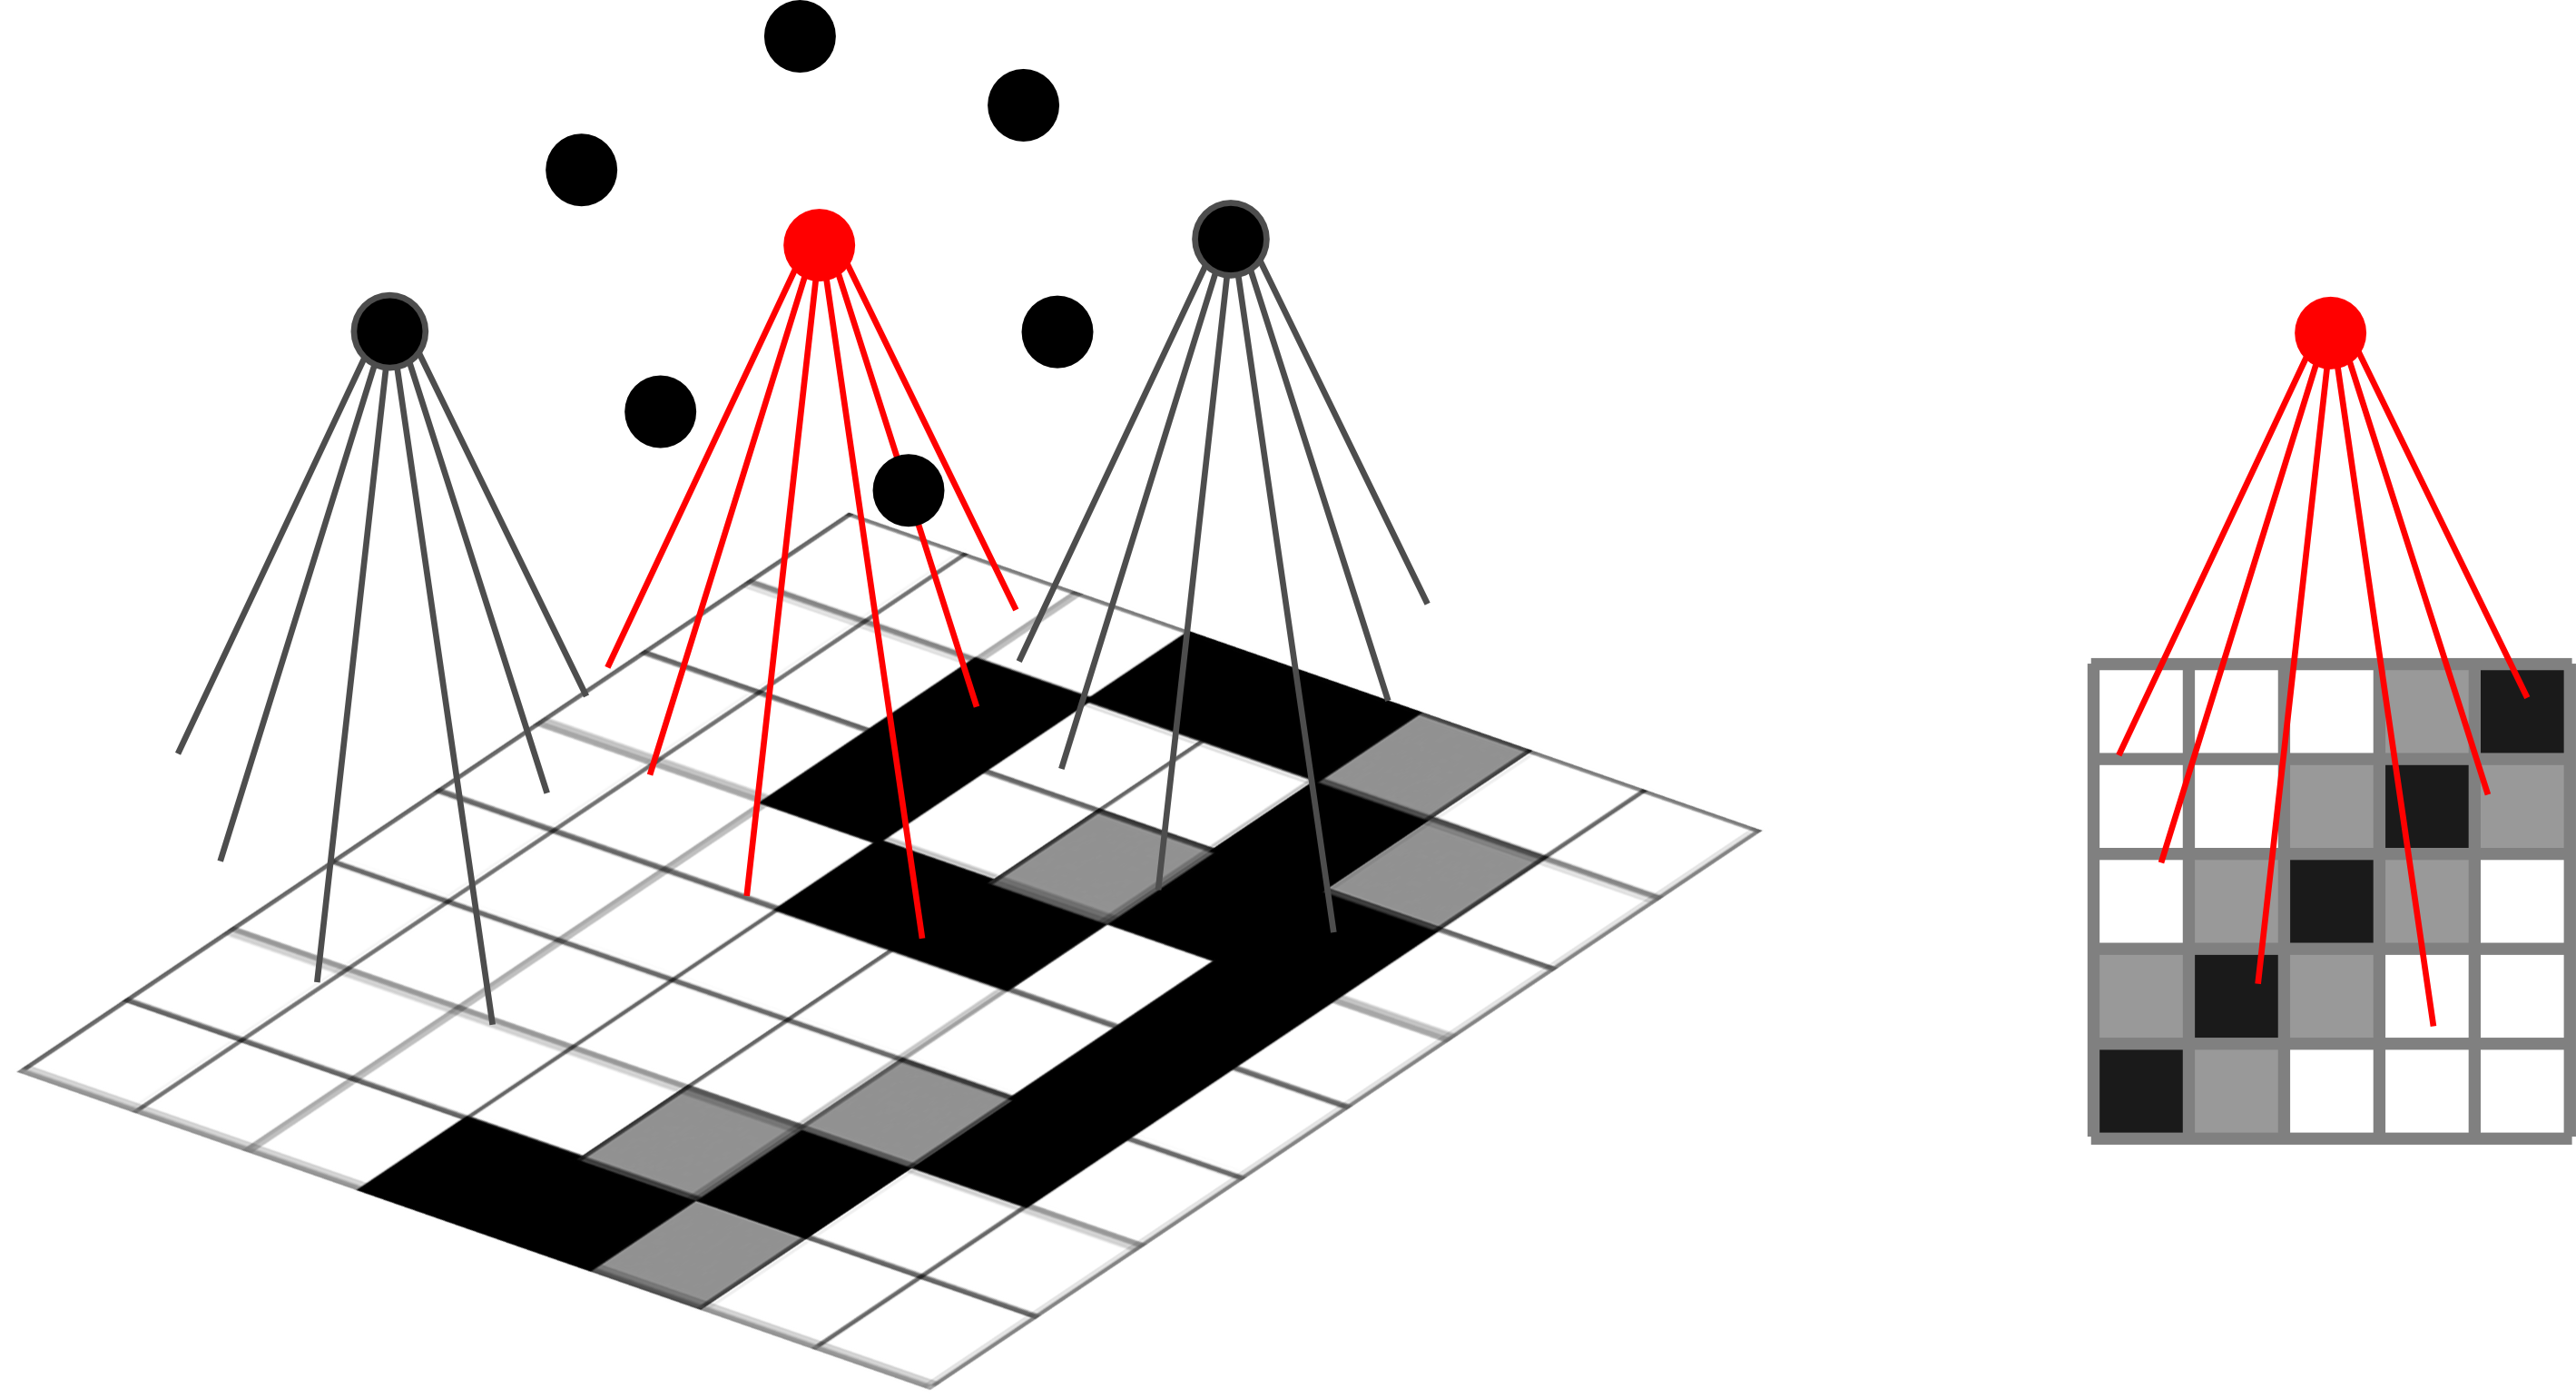
\includegraphics[scale=0.5]{feature-recognition.png}
\end{equation}
Suppose the red neuron is responsible for recognizing the ``diagonal line'' feature.  Its equation is $\vect{y} = \sigmoid (W \vect{x})$.  The matrix $W$'s role is to affine ``rotate'' the feature space, so that the features we desire is pointing in a certain direction.  Then we use $\sigmoid$ to ``\textbf{squeeze}'' the desired and undesired features.  The output after $\sigmoid$ represents the \textbf{presence or absence} of a particular feature, ie $\{0, 1\}$.  This is a form of information \textbf{compression}.

%假设红色的神经元专门负责辨识「对角线」这一特徵。 它的方程式是 $\vect{y} = \sigmoid (W \vect{x})$。  矩阵 $W$ 的作用是 affine「旋转」特徵空间,令我们想要的特徵指向某一方向。 然后再用 $\sigmoid$ 「\textbf{挤压}」想要的特徵和不想要的特徵。 Sigmoid 之后的输出,代表某类特徵的\textbf{存在与否},即 $\{0, 1\}$。 这是一种资讯的\textbf{压缩}。

%更准确地说,特徵被挤压到 $[0,1]$ 区间内,资讯没有消失,但如果计算的\textbf{解析度} (resolution) 有限,资讯确实会损失的。 如果输出层有 $n$ 个神经元,它们能够代表的 distributive features 个数是 $[0,1]^n$。 这是连续统的 $n$ 次幂,但解析度令它变成是有限的。

Let's digress a bit on \textbf{chaos theory}:  the role of $\sigmoid^{-1}$ is to ``stretch'', dragging points that are close neighbors to more distant positions.  Looking at the common \textbf{activation functions}, we see they are all non-linear \textbf{deformations} away from the identity $y = x$:
\begin{equation}
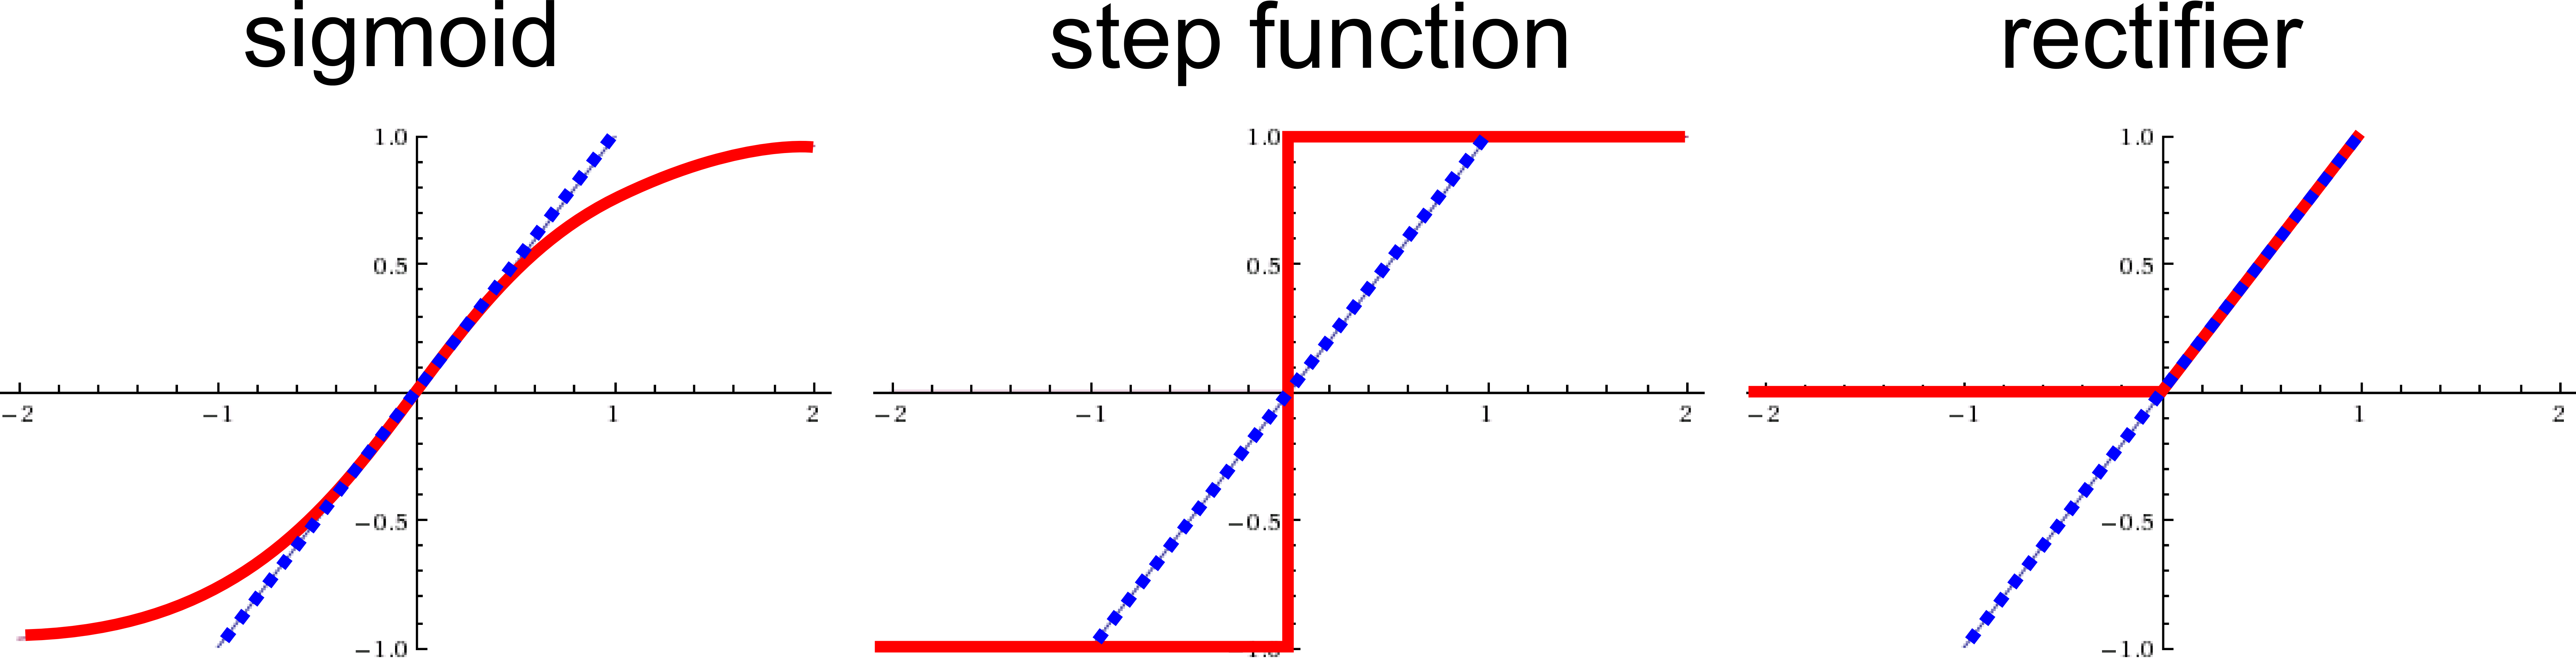
\includegraphics[scale=0.25]{activation-functions.png}
\end{equation}
This is very similar to the ``horseshoe'' proposed by Steven Smale \cite{Smale1967}, a recipe for creating chaos.  In other words, ``stretching'' and then putting back to the original space, and repeating this process, will create chaos \cite{Gilmore2011} \cite{Tel2006}. (The neural network running backwards in time has $\sigmoid^{-1}$, so its forward movement is also chaotic.)  A variant of the Smale horseshoe is the ``baker map'', analogous to kneading dough in bakery.
%这和 Steven Smale 提出的「马蹄」\cite{Smale1967} 非常类似,它是制造混沌的处方之一。 换句话说,「拉扯」然后放回原空间,如此不断重复,就会产生混沌 \cite{Gilmore2011} \cite{Tel2006}。 (神经网络的时间逆向就是 $\sigmoid^{-1}$,所以时间向前也是混沌。) Smale 马蹄的另一个变种叫做 baker map,其作用类似於「搓面粉」。

To summarize:\\
\underline{Each neuron represents the presence or absence of a certain \textbf{feature}.}\\
\underline{Higher-layer neurons represents \textbf{relations} between lower-layer features}.

%总结来说: \underline{每个神经元的输出代表某个 feature 的存在与否}。\\
%而,\underline{更高层的神经元代表下层 features 之间的\textbf{关系}}。

Following this line of thinking, we may conjecture this correspondence:
%凭这个思路推广,可以推测这样的 correspondence:
\begin{eqnarray}
\label{conclusion1}
\mathcal{M} & \quad \simeq \quad & \mathcal{X} \nonumber \\
\mbox{constant} \quad 
\includegraphics[scale=0.5]{node.png} & \quad \Leftrightarrow \quad & \mbox{neuron} \\
\mbox{relation} \quad 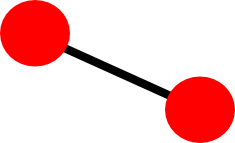
\includegraphics[scale=0.5]{link.png} & \quad \Leftrightarrow \quad & \mbox{relation between higher and lower neurons} \nonumber
\end{eqnarray}
But beware that this correspondence may not be 1-1, it could be one constant corresponding to several neurons' (linear?) \textbf{combination}.  The actual situation may be illustrated as follows (each layer may contain a vast number of neurons):
%但要注意的是这对应未必是一对一的,可能是一个 constant 对应几个 neurons 的\textbf{线性组合}。 具体情况可能像以下的示意图(实际上每层神经网络可能有很多神经元):
\begin{equation}
\label{conclusion2}
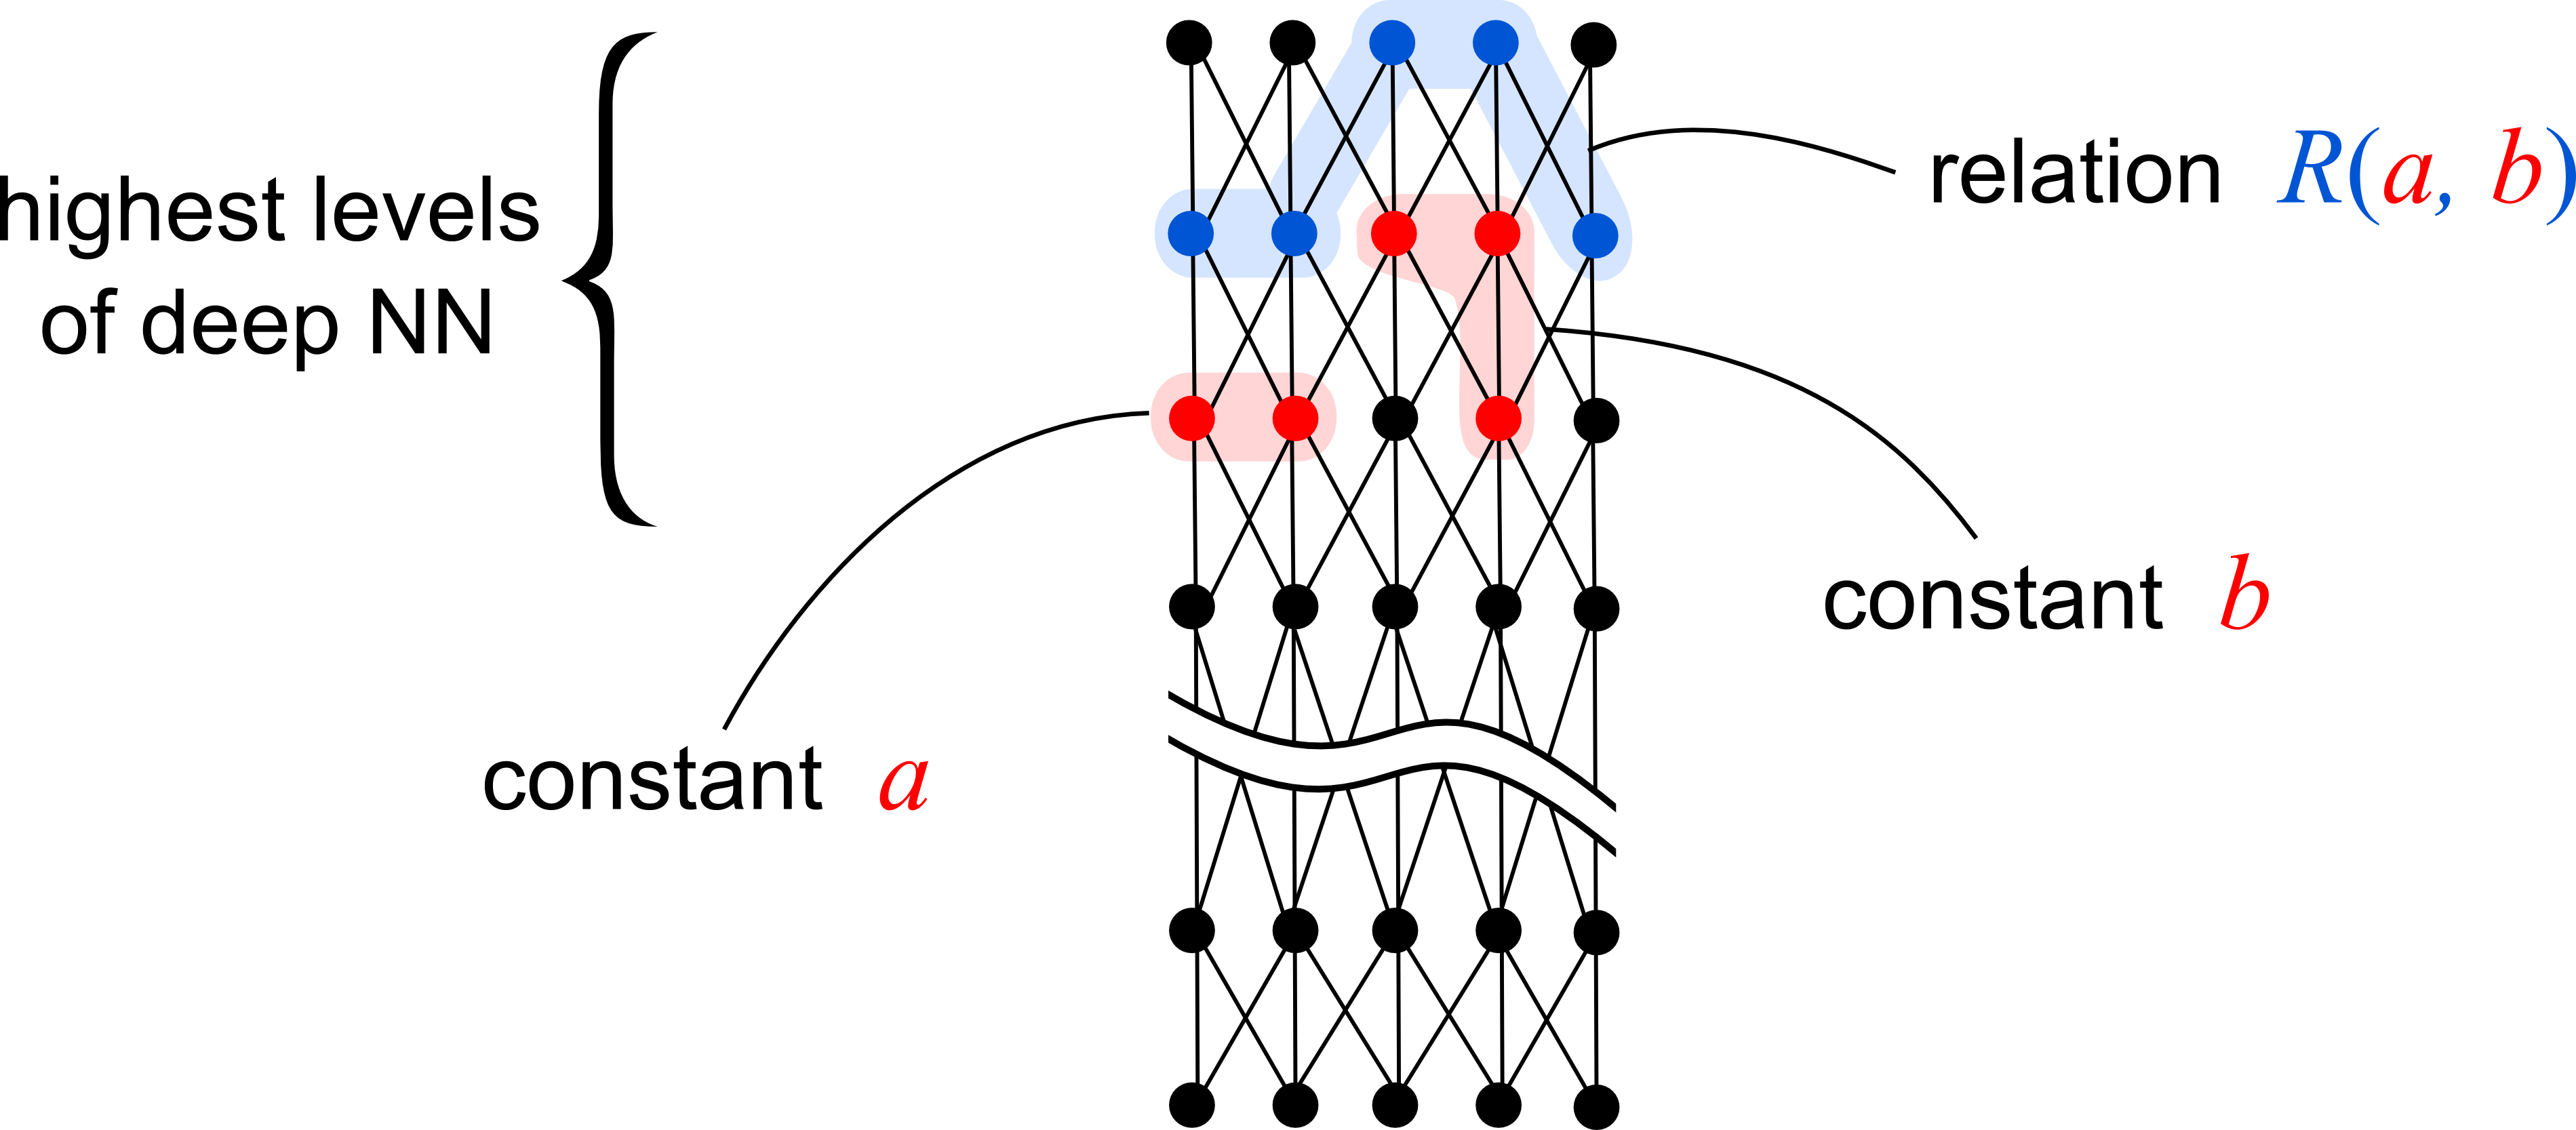
\includegraphics[scale=0.5]{actual-bridge.png}
\end{equation}
$R(a,b)$ can be searched for among the \textbf{common parents} of $a, b$ (eg. those blue neurons;  The value of $R(a, b)$ = a certain linear combination of blue neurons).  This can be verified by the condition:  If the signals of $a$ and $b$ are both ``present'', the value of $R(a, b)$ should also be ``true''.
%$R(a,b)$ 可以在 $a, b$ 的 common parents 中寻找(例如那些蓝色神经元,$R(a, b)$ 的值 = 蓝色神经元的某个线性组合)。  验证的方法是: 当 $a$ 和 $b$ 的信号都是「有」时,$R(a, b)$ 的值也应该是 true。 

\section{Conclusion}

This paper is not very successful because we have jumped to the conclusion  (\ref{conclusion1}) and (\ref{conclusion2}) without rigorous justification:  They are merely intuitively plausible.  In theory, since we have known how $\mathcal{M}$ is generated, and how $\mathcal{X}$ is generated, it should be feasible to build a ``highway'' between them.  In practice, it seems that we just need a deep neural network, because neural networks are \textbf{universal function approximators}, we don't even need to care about the structure between $\mathcal{M}$ and $\mathcal{X}$.

%这篇论文并不太成功,因为跳到 (\ref{conclusion1}) 和 (\ref{conclusion2}) 的结论没有严谨的根据,只是直观上觉得有可能。 理论上来说,既然知道了 $\mathcal{M}$ 那边是怎样生成的、$\mathcal{X}$ 那边是怎样生成的,则要在两边建立「高速公路」应该是可行的。 实际上,似乎只要建立一个深度网络就可以,因为神经网路是 universal function approximator,根本不用考虑 $\mathcal{M}$ 和 $\mathcal{X}$ 这两个结构之间的关系。

For further research, I hope some professional mathematicians can help with these problems:
%进一步的研究,希望数学专业的人能帮助一下:
\begin{enumerate}
\item On the logic side, could we transform its structure to one in \textbf{algebraic geometry}? In other words:  logic formulas $\simeq$ algebraic equations.  I only know of one instance of this kind of algebraic logic: Andreka \textit{et al}'s \cite{Andreka2001}, it seems to be an esoteric research area.
%\item 在逻辑那边,可不可以转换成 algebraic geometry 的结构? 即是说: 逻辑式子 $\simeq$ 代数方程。 这种代数逻辑的做法,我暂时只知道有 \cite{Andreka2001},是很偏门的研究。
\item From the structure of $\mathcal{M}$ and $\mathcal{X}$, can we find out the simplest form of a bridge between them?  Perhaps using mathematical induction, we examine the generative process of $\mathcal{M}$ and $\mathcal{X}$ layer by layer?
%\item 能不能根据 $\mathcal{M}$ 和 $\mathcal{X}$ 的结构,找出它们之间的桥的最简单形式?  可以用数学归纳法,逐步考虑 $\mathcal{M}$ 和 $\mathcal{X}$ 生成的方式,或许有帮助?
\end{enumerate}

%看上去颇复杂,但这样已经可以直接由逻辑式子 $\mathcal{L}$ 映射到深度网络的输出层。  在未有这理论之前,完全不知道这个 map 的结构;  但现在假如理论是正确的话,只需要简单的组合搜索 (combinatorial search) 就可以找到对应。  

\textbf{Application}:  When applying deep learning to natural language understanding, this theory may be helpful.
%应用: 对於用深度学习做 natural language understanding 的人,这理论或许会很有用。 

% Armed with this theory, we may construct an actual neuro-logic bridge.

\section{Prior art}

\begin{itemize}
\renewcommand\labelitemi{\textbullet}

\interfootnotelinepenalty=10000

\item Bader, Hitzler, H\"{o}lldobler and Witzel proposed in 2007 a method of neural-symbolic integration \cite{Bader2007}.  First they generate a Herbrand model\footnote{Herbrand model is a common construct in logic-based AI.  The gist is to generate from the logic language $\mathcal{L}$ ``whatever that can be instantiated'', resulting in an (often infinite) set of ground sentences (ie, without variables).  In other words, Herbrand models are generated from the language $\mathcal{L}$ self-reflexively, without relying on any external structure.  Every logic theory has at least one Herbrand model.} from the logic theory, maps the Herbrand model to a fractal space, and then directly use a neural network to learn that fractal space.  Though they used model theory, they did not make use of the correspondence between $\mathcal{M}$ and $\mathcal{X}$ in this paper.

%\item Bader, Hitzler, H\"{o}lldobler and Witzel 在 2007 年提出了一个 neural-symbolic integration 的做法 \cite{Bader2007}。 他们首先由 logic theory 生成抽象的 Herbrand model\footnote{Herbrand model 是邏輯 AI 中常用的概念,大意是用邏輯語言 $\mathcal{L}$ 生成「所有可以代入的東西」(instantiating whatever that can be instantiated),由此產生的不含變量的句子 (sentence) 的集合。 換句話說,Herbrand model 的特點是它只靠 $\mathcal{L}$ 自身產生它的模型,而不依賴任何外在結構。 每个邏輯 theory 都必然至少有一个 Herbrand model。},再将 Herbrand model 映射到某个 fractal 空间,然后直接用神经网络学习那 fractal 空间。  虽然用了 model theory,但他们没有利用到本文所说的 $\mathcal{M}$ 和 $\mathcal{X}$ 之间的关系。 

\item Khrennikov, in a series of papers starting from 1997, proposed using $p$-adic algebra to model the mental space $\mathcal{X}$, see his book co-authored with Anashin \cite{Anashin2009}.  A $p$-adic number can be regarded as a ``decimal'' number in base $p$, where $p$ is any prime.

\item Classical logic is binary;  There has been countless attempts to extend it to fuzzy or probablistic logic (eg. I have attempted in \cite{Yan2012}), but there is still not a unified concensus theory.  A slightly different approach, is to regard points in a space as first-order objects, and predicates as functions over that space.  Then we get a metric structure and on it a continuous first-order logic (CFOL) ~ \cite{Yaacov2008}.  This is a possible structure for $\mathcal{M}$.
%\item 经典逻辑是二元逻辑,近代已经有无数将它扩充到 fuzzy 或 probablistic 的尝试(作者也提出过 \cite{Yan2012}),但仍未有统一的理论。 与此不同的另一个方向,如果将点看成是 first-order objects,谓词是点空间上的函数,直接得到 metric structures 上的连续逻辑 (continuous first-order logic) ~ \cite{Yaacov2008},这可以看成是一种 $\mathcal{M}$ 的结构。

\item In model theory there  are ultra-filters and ultra-products, which originated in functional analysis.  Recently there has been novel research crossing between model theory and Banach space \cite{Iovino2002}.  Simply put, the ultra-product is a way to multiply existing models to yield new models.  I looked at it briefly and found that ultra-products often involve sets of infinite cardinality and are very ``big'' constructs.  So they may not be very practical for computational implementation.

\end{itemize}

\section*{Acknowledgement}

\footnotesize{Thanks to Ben Goertzel for discussions on the AGI mailing list.  Ben first pointed out the advantage of neural network learning over inductive logic learning, which prompted me to research their relationships.  Thanks also to Juan Carlos Pinto for personal discussions on the structure of neural networks.}

% =====================================================================================
\begin{comment}
\section{逻辑变量的处理}

这可能是最辣手的部分。

Alfred Tarski 提出了 cylindrical algebra 来解决「一阶谓词逻辑」的变量问题,但据说 Tarski 自己也觉得 cylindrical algebra 「不好用」。 我觉得它比较难明,从略。

个人觉得比较好的做法是 Paul Halmos 的 algebraic logic。 其中最关键的建构是:
\renewcommand\labelitemi{--}
\begin{eqnarray}
\mbox{谓词} : \mbox{物体} & \rightarrow & \mbox{命题空间} \nonumber \\
\cancel\heartsuit : \cancel\heartsuit(\mbox{john}) & \mapsto & \mbox{「阿 John 失恋」} \nonumber \\
\cancel\heartsuit : \cancel\heartsuit(\mbox{pete}) & \mapsto & \mbox{「阿 Pete 失恋」}
\end{eqnarray}
换句话说,predicate(谓词)就是一些将 object (逻辑中的物体,或「常项」,constants)映射到个别命题的\textbf{函数}。 这些谓词函数可以有一个或多个\textbf{参数},分别叫 monadic 和 polyadic predicate calculus。

最新的逻辑代数化方法来自\textbf{範畴论},William Lawvere 在 1960's 年代提出(也就是 \textit{Conceptual Mathematics} 这本书的作者之一)。  他发现了 $\forall$ 和 $\exists$ 是 adjoint functors 的关系; 这个 adjunction 比较难懂,有兴趣可以看 \cite{Lawvere2003}。
\end{comment}
% =====================================================================================

\bibliographystyle{plain} % or number or aaai ...
\bibliography{AGI-book}

\end{document}